\documentclass{aastex631}
\usepackage{amsmath}
\usepackage{amssymb}
\usepackage{hyperref}
\usepackage{bm}
\usepackage{listings}
\usepackage{graphicx}
\usepackage{float}

% commands
\newcommand{\nuance}{\texttt{nuance}}
\newcommand{\TODO}{\texttt{todo}}
\newcommand{\set}[1]{\{\,#1\,\}}
\newcommand{\footlink}[1]{\footnote{\url{#1}}}
\newcommand{\wtls}{\texttt{biweight+BLS}}
\DeclareMathOperator*{\argmax}{arg\,max}
\DeclareMathOperator*{\argmin}{arg\,min}

% no indent
\setlength\parindent{0pt}

% code style
\lstdefinestyle{mystyle}{
    backgroundcolor=\color{white},
    commentstyle=\color{gray!70},
    keywordstyle=\color{Bittersweet},
    stringstyle=\color{RoyalBlue},
    basicstyle=\fontsize{7.5}{11}\fontfamily{DejaVuSansMono-TLF}\selectfont,
    breakatwhitespace=false,         
    breaklines=true,
    rulecolor=\color{black!15},
    numbers=none,
    numberstyle=\fontsize{7}{11}\fontfamily{DejaVuSansMono-TLF}\selectfont\color{gray!50},
    framerule=0pt,
    breakindent=5pt,
    resetmargins=true,
    numbersep=10pt,
    frame=single,
    aboveskip=1em,
    belowskip=1em,
    xleftmargin=6pt,
    framexleftmargin=4pt
}
\lstset{style=mystyle}

% figure options
\graphicspath{{../figures}}

\begin{document}

\title{\texttt{nuance}: Detection of planetary transits in the presence of correlated noise}

% author info
\author{Lionel J. Garcia}
\author{Daniel Foreman-Mackey}
\affiliation{Center for Computational Astrophysics, Flatiron Institute, New York, NY, USA}
\correspondingauthor{Lionel J. Garcia}
\email{lionel\_garcia@live.fr}

\begin{abstract}
    We present \texttt{nuance}, an algorithm to search for planetary transits in light curves featuring correlated noise, such as instrumental signals and stellar photometric variability. To deal with these nuisance signals, a common approach consists in cleaning a light curve from correlated noise before searching for transits. However, we show that this approach, based on the prior assumption that transits are not present, strongly degrades their signals, up to the point of no detection. As this degradation depends on the correlated noise characteristics, we explore the parameter space for which transits are altered, and quantify this effect on a wide variety of cases. We show that \nuance{} outperforms the detection capabilities of commonly used transit search algorithms, especially for light curves featuring correlated noise with an amplitude three times greater than the searched transit depth. We perform our tests by injecting transits on synthetic light curves, and on known TESS candidates light curves to assess the performance of our algorithm on realistic multi-planetary systems datasets. Beyond its detection efficiency, we make \nuance{} tractable, \TODO{} times faster than current alternatives based on brute force detrending, and available as a well documented open-source Python package\footnote{\href{https://github.com/lgrcia/nuance}{https://github.com/lgrcia/nuance}}.
\end{abstract}

\section*{Introduction}
Transiting exoplanets are keystone objects for the field of exoplanetary science, but detecting transits in light curves featuring stellar variability and instrumental signals remains a challenge \citep{Pont2006,Howell2016}. For this reason, known transiting exoplanets tend to be found around quieter stars, or belong to the population of close-in giants whose transit signals dominate over stellar rotational variability \citep{Simpson2023}. However, discovering transiting exoplanets around active stars holds few promises. First, as younger stars are more active\footnote{approximately down to spectral type MV ()} \citep{Skumanich1972}, being able to detect planets transiting active stars will favor the discovery of young planetary systems \citep[e.g.][]{Newton2022}. Second, as stellar variability may originate from surface active regions (such as starpots), the increased discovery of occulting companions will increase our chances to map the photosphere of active stars \citep[e.g.][]{Morris2017}, benefiting both the study of stellar atmospheres and the concerning impact of their non-uniformity on planetary atmosphere retrievals \citep{rackham2018}. Overall, enabling the detection of transits in light curves with high levels of correlated noises will greatly benefit the study of terrestrial exoplanets around late M-dwarfs, usually observed at lower SNR and more likely to display photometric variability (e.g. \citealt{Murray2020}).
\\\\
Commonly used transit-search algorithms, such as the Box-Least-Square algorithm \citep[BLS,][]{bls} are capable of detecting transits in light curves containing only transit signals and white noise. Using this method, the simplest way to detect transits in a light curve featuring correlated noise (either astrophysical or instrumental), is to first clean it from nuisance signals before performing the search. This strategy is widely adopted by the community, both using physically-motivated systematic models like \cite{everest1, everest2}, or filtering techniques (\citealt{Jenkins2010}, \citealt{wotan}). However, when correlated noise starts resembling transits, this cleaning step (often referred to as \textit{detrending}) is believed to degrade their detectability \cite[see subsection 4.3 of][]{wotan}. In this case, the only alternative to search for transits is to perform a full-fledged modeling of the light curve, including both transits and correlated noise, and to compute the likelihood of the data to the transit model on a wide parameter space (an approach largely avoided due to its intractable nature). Nonetheless, \cite{kovacs2016} ask: \textit{Periodic transit and variability search with simultaneous systematics filtering: Is it worth it?}. The latter study explores a handful of cases and generally discards the benefit of using a full-fledged approach. However, it does not explore the light-curves characteristics for which such a complete modeling becomes necessary.
\\\\
In this paper, we explore the light curve characteristics for which a full-fledge transit search is necessary, an we present \nuance{}, a method to search for transit signals while modeling correlated noises in a tractable way. 

\section{The degradation of transit detectability}\label{issues}

A strong assumption when using BLS-type algorithms is that the searched dataset only contains transit signals and white noise. Hence, two sources of correlated noise particularly justify the need for a detrending step before searching for transits: instrumental signals (such as those induced by telescope pointing errors) and astrophysical signals (such as stellar variability induced by pulsations or starspots). In this section, we qualitatively study the effect of correlated noise and its detrending on transits detectability.

\subsection{Transit detectability}

One way to study the detectability of a unique transit signal is to compute its signal-to-noise-ratio (SNR, \citealt{Pont2006}, Equation 12):
\begin{equation}\label{eq:snr}
  SNR= \frac{\Delta}{\sqrt{\frac{\sigma_w^2}{n} + \frac{\sigma_c^2}{N_{tr}}}}
\end{equation}
where $\Delta$ is the relative transit depth, $n$ is the number of points within transit, $N_{tr}$ the number of transits ($N_{tr}=1$ here), and $\sigma_w^2$ and $\sigma_c^2$ are the white and correlated noise variances. \autoref{fig:issue1} shows this metric computed for a unique transit observed in the absence (grey) and presence (red) of correlated noise.

\begin{figure}[H]
    \begin{centering}
        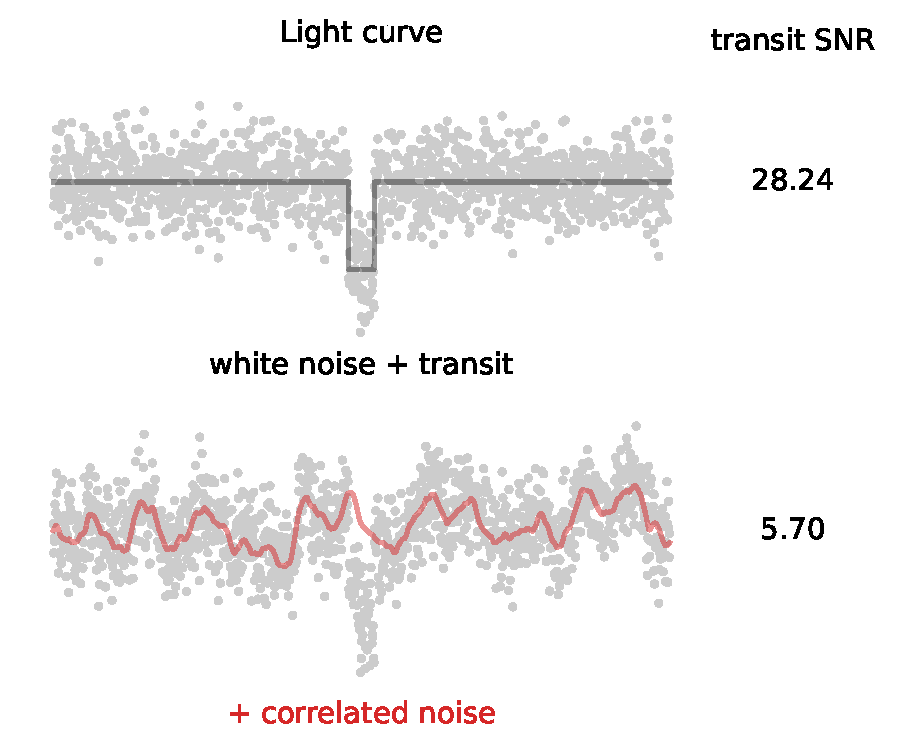
\includegraphics[width=8.5cm]{issue1.pdf}
        \caption{Illustration of the effect of correlated noise on a single transit SNR. A 1-hour transit signal of depth 1\% is generated on top of white noise (variance of $0.0015^2$) as part of a 24-hours observation with an exposure time of 1 minute (top). Then, in the bottom plot, correlated noise is added, generated using a Gaussian Process with a Matèrn-32 kernel of scale 1 hour and sigma of 0.2\%. The SNR on the right of each light curve is computed using \autoref{eq:snr}. Models used to simulate these data are provided in \autoref{signals_simulations}.}
        \label{fig:issue1}
    \end{centering}
\end{figure}

As illustrated in \autoref{fig:issue1}, the presence of correlated noise strongly decreases the transit signal SNR, which would ultimately limit its detectability. 

\subsection{Detrending methods and their effects}\label{detrending_effect}
The presence of instrumental correlated noise motivated the development of systematics detrending algorithms, such as the Trend Filtering Algorithm (\textsc{TFA}, \citealt{tfa}, in its primary use case), \textsc{SysRem} (\citealt{sysrem}) or Pixel Level Decorrelation (\textsc{PLD}, \citealt{pld}; see also \textsc{Everest} from \citealt{everest1, everest2}). Most of these methods rely on the shared nature of instrumental signals among light-curves (or neighboring pixels) such that the correction applied should not degrade the transit signal and can be modeled using contemporaneous measurements (like detector's temperature, pointing error, sky background or airmass time series). In opposition, stellar variability and other astrophysical signals cannot be correlated with simultaneous measurements. This gave rise to several treatments in order to reconstruct and detrend stellar variability. One of them is physically-motivated and makes use of Gaussian processes (e.g. \citealt{k2sc}), another is empirical and makes use of filtering algorithms (\citealt{Jenkins2010}, \citealt{wotan}).

\begin{figure}[H]
    \begin{centering}
        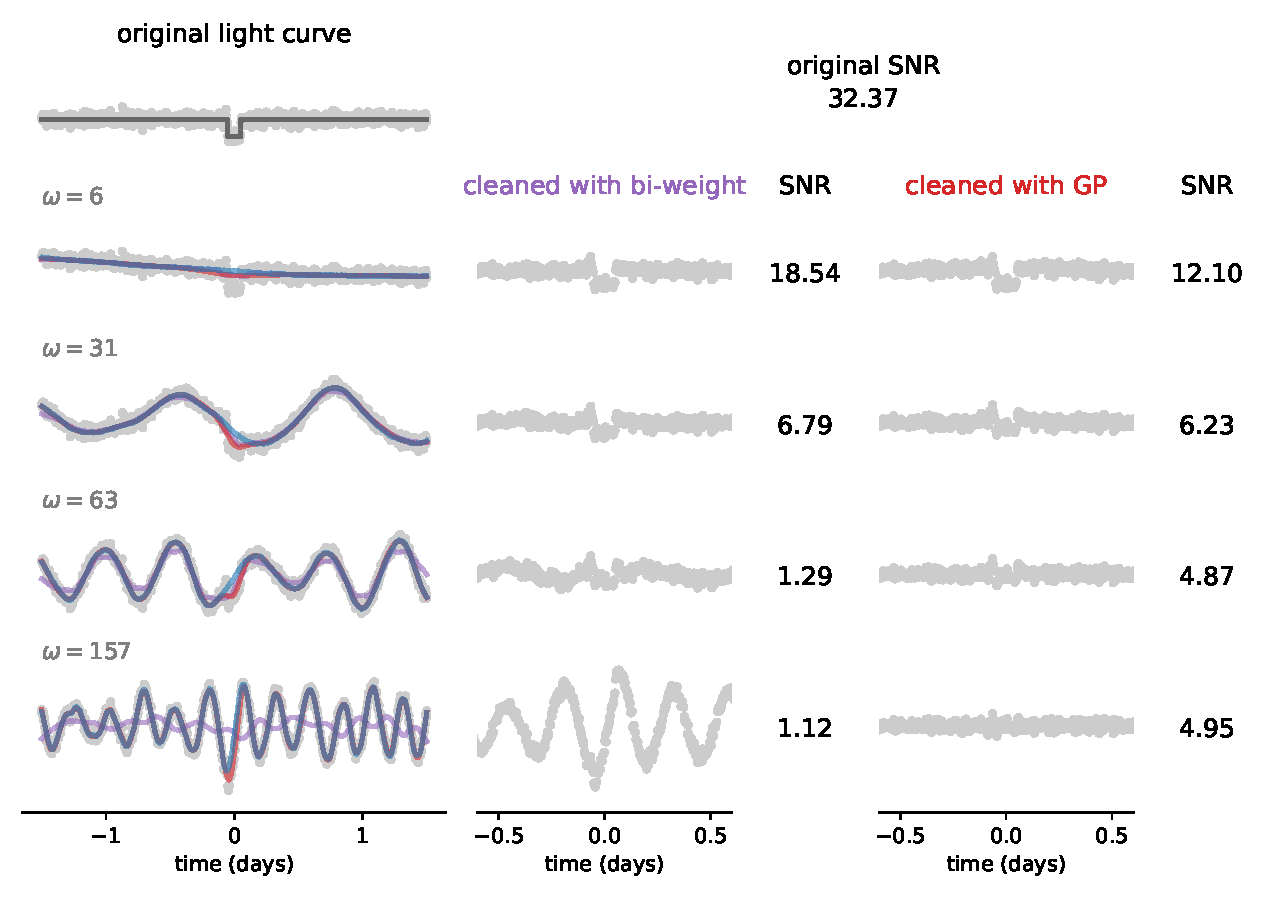
\includegraphics[width=0.85\linewidth]{issue2.pdf}
        \caption{(Top left) Simulated observation spanning 3 days, including a transit signal with a depth of 0.8\%, duration of 0.1 day, and measurement error of 1.5\% (using the model from \cite{protopapas} described in \autoref{app_proto}). (Left) Correlated noise in the form of stellar variability with different timescales and amplitudes added to the unique transit signal. This signal is then reconstructed using (in purple) Tukey's bi-weight filter \citep{wotan} with an optimal window size of three times the transit duration, and (in red) a Gaussian Process with the same kernel used to simulate the data. In each case the variability is reconstructed, subtracted, and the transit SNR computed using \autoref{eq:snr} with the transit depth estimated as the minimum in-transit flux.}
        \label{fig:issue2}
    \end{centering}
\end{figure}

In \autoref{fig:issue2}, we simulate a transit signal on top of which we add photometric stellar variability with different amplitudes and timescales, sampled from a Gaussian Process with an SHO kernel described in \autoref{app_gp}. For each light curve, we reconstruct and detrend stellar variability in two ways: one using the widely-adopted Tukey's bi-weight filter, presented in \cite{tukey} and using the implementation from \textsf{wõtan}\footnote{\href{https://github.com/hippke/wotan}{https://github.com/hippke/wotan}} \citep{wotan}; the other using the same Gaussian Process from which the data has been sampled. We then estimate the resulting transit depth and compute the remaining transit SNR using \autoref{eq:snr}. 

\noindent \autoref{fig:issue2} clearly shows the effect of both detrending techniques on transits SNR, and intuitively suggests that the degradation is strongly dependant on the correlated noise characteristics encountered.\\\\
In order to explore the parameter space for which detrending is the most problematic, we employ the method previously described to simulate 10 000 light curves containing a transit signal and correlated noise in the form of stellar variability. For each light curve, we reconstruct the variability signal and detrend it using an optimal bi-weight filter before estimating the remaining transit SNR. For convenience, the simulated light curves share a common transit added on top of white noise, and a variability signal only defined by two parameters: $\tau$, the relative timescale of the variability with respect to the transit duration; and $\delta$, the relative amplitude of the variability against transit depth, corresponding to an SHO kernel with hyperparameters chosen as: 
\begin{equation}\label{eq:relative_params}
    \omega = \frac{\pi}{\tau D}, \hspace{0.5cm} 
    \sigma = \delta \frac{\Delta}{2} \hspace{0.5cm}  \text{and}  \hspace{0.5cm}  
    Q = 10,
\end{equation}
with $\Delta=1\%$ and $D=0.04$ days, the depth and duration of the simulated transit. 
% We fix a relatively high value for the quality factor $Q$ in order to restrict our simulations to strongly periodic variability signals. 

For $\tau=1$ and $\delta=1$, the expressions of $\omega$ and $\sigma$ given in \autoref{eq:relative_params} correspond to a variability signal with a period half that of the transit duration, and a standard deviation two times that of the transit depth, i.e. strongly resembling the simulated transit signal.

\autoref{fig:snr_detrend} shows that it exists an entire region of the $(\tau, \delta)$ parameter space for which the bi-weight detrending degrades transit SNR to the point of no detection ($SNR < 6$). Hence, bi-weight filter detrending makes transit-search blind to many systems. While this study should be extended to other detrending techniques, it highlights the need for a more informed transit search algorithm able to deal with correlated noise.


\begin{figure}[H]
    \begin{centering}
        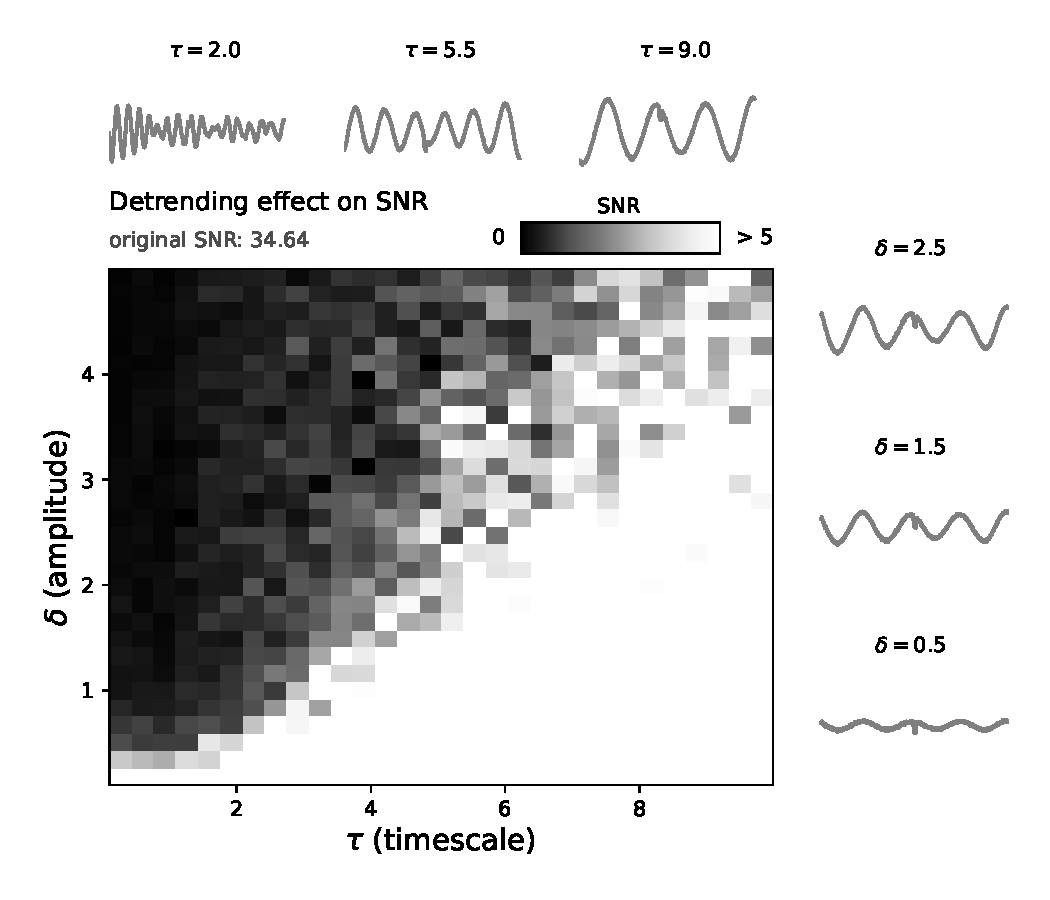
\includegraphics[width=0.7\linewidth]{../workflows/cleaning_snr/figures/result.pdf}
        \caption{SNR of a unique transit after detrending light curves using an optimal bi-weight filter. All light curves correspond to a 2.8 days observation with a cadence of 2 minutes, and contain a unique transit of duration 1 hour and a depth of 1\%, added on top of white noise with a standard deviation of 0.5\% plus stellar variability. Light curves at the top and right side of the central plot are shown with their corresponding $\tau$ and $\delta$ values. The amplitude of the variability increases with $\delta$ and the timescale of the variability increases with $\tau$.}
        \label{fig:snr_detrend}
    \end{centering}
\end{figure}


\newpage
\section{\textsf{nuance}}\label{nuance}

\textsf{nuance} is an algorithm capable of searching for planetary transits in light curves containing correlated noise, such as instrumental signals and photometric stellar variability.
\\\\
Let assume that the flux $f$ of a star is observed and arranged in the vector $\bm{f}$ of size $N$, associated to the vector of times $\bm{t}$. This flux, shown in \autoref{fig:linear_search}, contains instrumental signals, stellar variability and a periodic transit signal that we wish to uncover. We assume that a set of $M$ observed measurements (such as the position of the star on the detector or the sky background) taken at the same time as the flux can be treated as explanatory variables for $\bm{f}$. These measurements constitute the columns of the $(N\times M)$ \textit{design matrix} $\bm{X}$.\\\\

Ideally, we would detect the periodic transit signal in this flux by sampling the posterior likelihood of this data to a full-fledge model including stellar variability (more generally correlated noise), instrumental systematic signals (modeled with explanatory variables or treated as correlate noise), and a periodic transit signal of period $P$, epoch $T_0$, duration $D$ and depth $\Delta$. We would then reduce the posterior likelihood to $p(\bm{f}\vert P)$, its marginalized version over all parameters except the period $P$, producing a transit search periodogram $\mathcal{Q}(P)$. However, this approach has two issues: It is highly intractable, and it may lead to multimodal distributions that are hard to interpret.
\\\\
Given a period $P$, we instead want to compute the likelihood of a periodic transit signal at the maximum likelihood parameters $\hat T_0$, $\hat D$ and $\hat \Delta$, i.e the periodogram
\begin{equation}\label{eq:periodogram}
        \mathcal{Q}(P) = p(\bm{f} \vert P, \hat T_0 ,\hat D, \hat \Delta)
\end{equation}
This is done by adopting the strategy of \cite{foreman2016}, and separate the transit search into two components: the linear search and the periodic search. During the linear search, the likelihood of a single non-periodic transit is computed for a grid of epochs, durations and depths. Then, the periodic search consists in combining these likelihoods to compute the likelihood of the data given a periodic transit signal for a range of periods. These combined likelihoods yield a transit-search periodogram on which the periodic transit detection is based. \textsf{nuance} differs from \cite{foreman2016} and other existing transit search algorithms as it models the covariance of the light curve with a Gaussian Process, accounting for correlated noise (especially in the form of stellar variability) while keeping the model linear and tractable. This way, \textsf{nuance} searches for transits while, at the same time, modeling correlated noise, avoiding the detrending step that degrades transit signals SNR.\\\\
We note that the approach employed by \textsf{nuance} (using the two steps proposed by \citealt{foreman2016}), shares similarities with the approach of \cite{Jenkins2010}, where a single event statistic is computed and combined into a multiple event statistics.

\subsection{The linear search}\label{linear_search}

During the linear search, the goal is to compute the likelihood $p(\bm{f} \vert T , D, \Delta)$ of the data given a single non-periodic transit signal of epoch $T$, duration $D$ and depth $\Delta$, for a grid of epochs, durations and depths.
\\\\
To account for correlated noise, the light curve $f$ is modeled as being drawn from a Gaussian Process, like the simulated light curves used in \autoref{issues}, such that
\begin{equation*}
    \bm{f} \sim \mathcal{N}(\bm{X w}, \bm{\Sigma}),
\end{equation*}
with mean $\bm{Xw}$ (i.e. a linear model of the M explanatory variables with coefficients $\bm{w}$) and covariance $\bm{\Sigma}$. To account for the presence of a single non-periodic transit of epoch $T$ and duration $D$, this signal is computed and appended as the last column of the design matrix $\bm{X}$, using the simple transit model from \cite{protopapas} with a unitary depth (\autoref{eq:protopapas}). This way, the transit signal is part of the linear model and its depth $\Delta$ can be solved linearly. Under this assumption, the log-likelihood of the data given a single non-periodic transit is \citep{Rasmussen2005}
\begin{equation} \label{eq:linear_search_ll}
    \ln p(\bm{f} \vert I) = -\frac{1}{2}(\bm{f}-\bm{Xw})^T\bm{\Sigma}^{-1}(\bm{f}-\bm{Xw}) -  \frac{1}{2}\ln\vert\bm{\Sigma}\vert - \frac{N}{2}\ln 2\pi,
\end{equation}
where the parameters vector $\bm{w}$ and their errors $\bm{\sigma}$ are computed using the generalized least-square solution
\begin{equation}\label{eq:ls}
    \bm{w} = (\bm{X}^T\bm{\Sigma}^{-1}\bm{X})^{-1}\bm{X}^T\bm{\Sigma}^{-1}\bm{f} \hspace{0.5cm} \text{and} \hspace{0.5cm} \bm{\sigma} = (\bm{X}^T\bm{\Sigma}^{-1}\bm{X})^{-1},
\end{equation} 
with $\bm{\Sigma}$ the covariance matrix modeled using the Gaussian Process. Hence, $\ln p(\bm{f} \vert I)$ can be computed on a grid of epochs and durations, the transit depth being linearly solved for any $(T, D)$. In this equation. This linear search leads to the set of likelihoods
\begin{equation*}
    \set{\ln\mathcal{L}_{i,j}}_{i, j} = \set{\ln p(\bm{f} \vert T_i ,D_j, \Delta_{i,j})}_{i, j},
\end{equation*}
were $\Delta_{i,j}$ is the depth linearly solved for a given $(T_i, D_j)$\footnote{The expression of $\set{\ln\mathcal{L}_{i,j}}_{i, j}$ omits the vector $\bm{w}_{i,j}$ (except its last value $\Delta_{i,j}$) as it is also linearly solved for any given value of $(T_i, D_j)$ and irrelevant in what follows.}. \autoref{fig:linear_search} shows this likelihood grid computed for a simulated dataset, using the same Gaussian Process  and design matrix $\bm{X}$ used to simulate the data.

\begin{figure}[H]
    \begin{centering}
        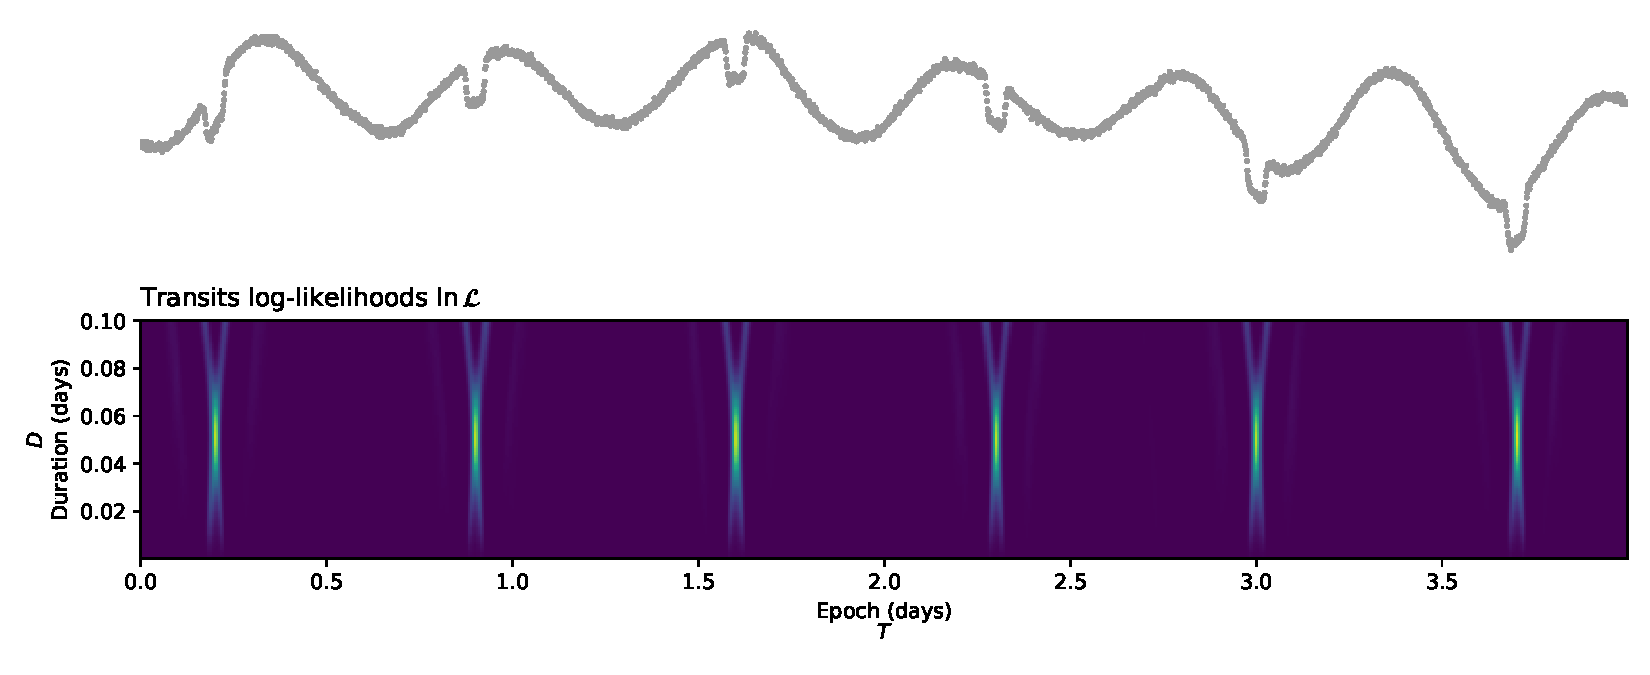
\includegraphics[width=0.8\linewidth]{principle_linear_search.pdf}
        \caption{Principle and output of the linear search. The simulated dataset (top) corresponds to the one shown and described in \autoref{fig:app_principle_dataset}. First, a set of durations and depths $\set{T_i, D_j}_{i,j}$ is generated. For each pair of indices $(i,j)$, the likelihood $\ln p(\bm{f} \vert T_i ,D_j, \Delta_{i,j})$ is computed using the parameters from \autoref{eq:ls} and the expression of \autoref{eq:linear_search_ll}. This process yields the grid of log-likelihoods $\ln\mathcal{L}$ (bottom plot), as well as the $\set{\Delta_{i,j}, \sigma_{i,j}}_{i, j}$ transit depths and errors inferred linearly using \autoref{eq:ls}.}
        \label{fig:linear_search}
    \end{centering}
\end{figure}

\noindent To prepare for the next step, the corresponding depths $\Delta_{i,j}$ linearly solved for any $(T_i ,D_j)$ are stored, as well as their associated uncertainties $\sigma_{i,j}$, corresponding to
\begin{equation*}
    \Delta_{i,j} = \bm{w}_M \hspace{0.5cm}\text{and}\hspace{0.5cm} \sigma_{i,j} = \bm{\sigma}_{MM},
\end{equation*}
M denoting the index of the last column of the design matrix $\bm{X}$, where the transit signal is contained.

\subsection{The periodic search}

We then need to combine the likelihoods computed from the linear search to obtain
\begin{equation*}
    p(\bm{f} \vert P, T_0 , D, \Delta),
\end{equation*}
i.e.\,the probability of a periodic transit of period $P$, epoch $T_0$, duration $D$ and depth $\Delta$ given the data $\bm{f}$. For a given transit duration $D$, any combination of $(P, T_0)$ leads to K transits, for which it is tempting to write
\begin{equation}\label{eq:attempt}
    p(\bm{f} \vert P, T_0 ,D, \Delta) = \prod_k^K p(\bm{f} \vert T_k, D, \Delta_k),
\end{equation}
where $\set{T_k}_k$ are the epochs matching $(T_0, P)$ and $\set{\Delta_k}_k$ the corresponding depths. So that
\begin{equation*}
    \ln p(\bm{f} \vert P, T_0 ,D, \Delta) = \sum_k^K \ln \mathcal{L}_k.
\end{equation*}
This is the joint likelihood of transits belonging to the same periodic signal but with varying depths  $\set{\Delta_k}_k$. However, individual transits from a periodic signal cannot be considered independent, and should instead be found periodically and share a common transit depth $\Delta$. To this end, it can be shown (see \autoref{proof}) that there is an analytical expression for the joint likelihood of K individual transits with depths and errors $\set{\Delta_k, \sigma_k}_k$ assuming a common depth $\Delta$, corresponding to 
\begin{equation}\label{eq:result}
    \begin{gathered}
        \ln p(\bm{f} \vert P, T_0 ,D, \Delta) =  \sum_{k}^K \ln \mathcal{L}_k  - \frac{1}{2} \sum_k^K\left(\ln(\sigma_{k}^2) - \ln(\sigma^{2} + \sigma_{k}^{2}) +  \frac{\left(\Delta_{k} -
        \Delta\right)^{2}}{\sigma_k^{2} + \sigma^{2}}\right) \\
        \text{with} \quad  \frac{1}{\sigma^2} = \sum_k^K \frac{1}{\sigma_k^2} \quad \text{and} \quad
        \Delta = \sigma^2 \sum_k^K {\frac{\Delta_k}{\sigma_k^2}}.
    \end{gathered}
\end{equation}

While \autoref{eq:result} takes a closed form, the individual epochs matching $T_0$ and $P$ are not necessarily available in the grid of epochs $\set{T_k}_k$. In \cite{foreman2016}, a similar issue is solved by using the nearest neighbors in the epochs grid. Instead, to allow the efficient matrix computation of \autoref{eq:result}, the likelihood grid is linearly interpolated from $\set{T_i}_i$ to a common grid of transit phases $\set{\phi_i}_i$, leading to the periodic search log-likelihood
$$\ln\mathcal{P}(P) = \set{\ln p(\bm{f} \vert P, \phi, D)}_{i,j}$$
shown for few periods in \autoref{fig:periodic_search} (b). In the latter equation, $\Delta_{i,j}$ is omitted since being interpolated from the linear search using $\phi_i$, $D_j$ and $T_0 = 0$.

\begin{figure}[H]
    \centering
    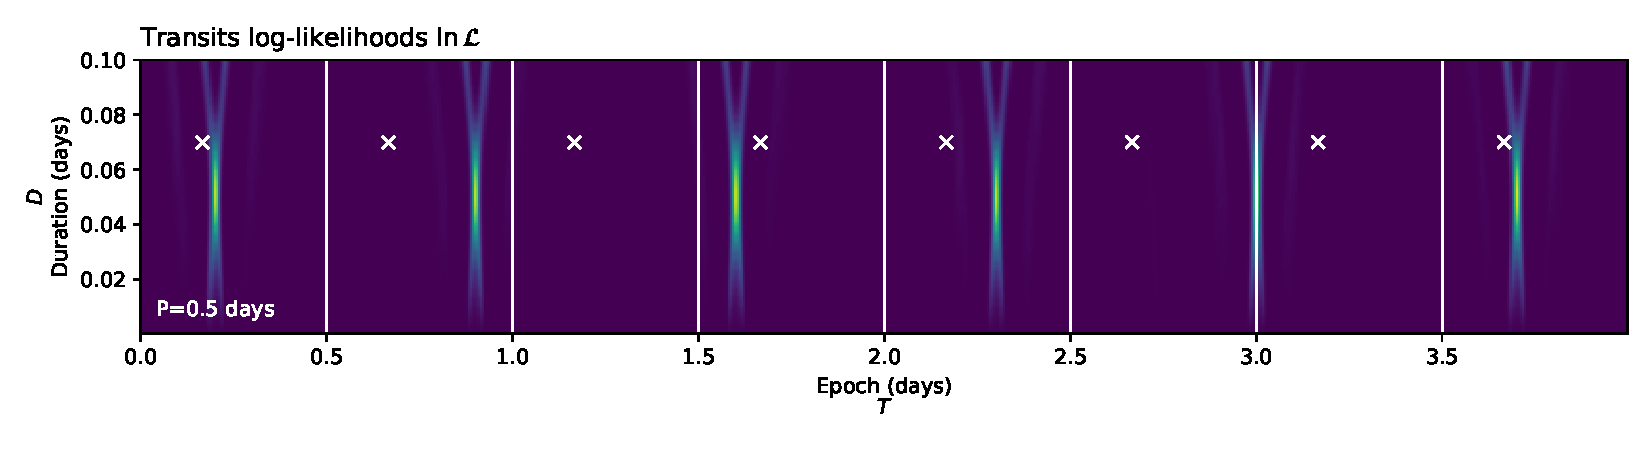
\includegraphics[width=0.8\linewidth]{principle_periodic_0.pdf}\\
    {(a) $\ln \mathcal{L}$}

    \centering
    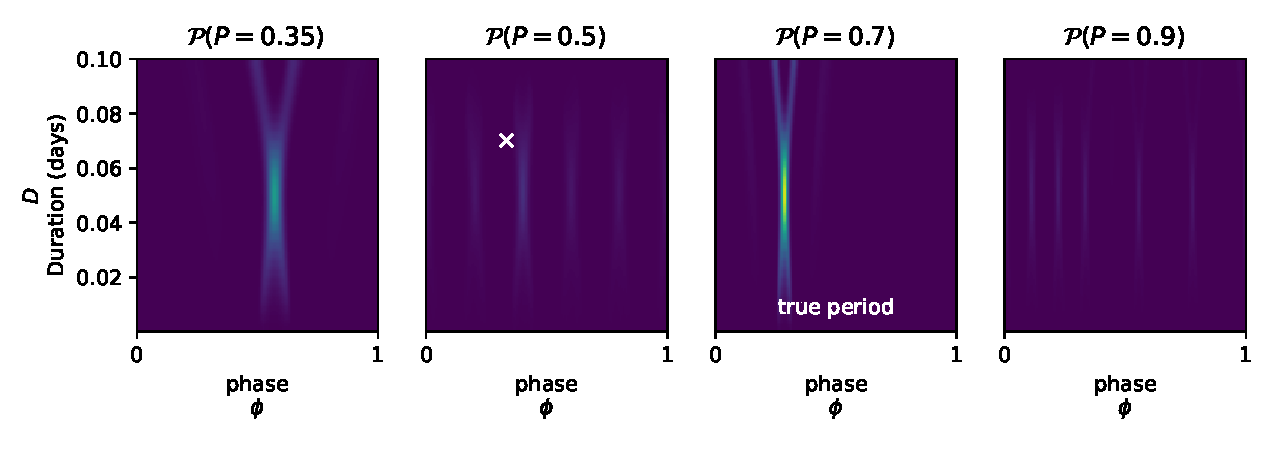
\includegraphics[width=0.8\linewidth]{principle_periodic_1.pdf}\\
    {(b) $\mathcal{P}(P)$}
\end{figure}

\begin{figure}[H]
    \caption{Applied to the dataset shown \autoref{fig:linear_search}, this figure shows how the periodic search works at different periods $P$ (including the true period $P = 0.7$ days). Given different periods $P$ and $T_0=0$, the likelihood $\ln\mathcal{L}$ shown in (a) is phase-folded and interpolated onto a common grid of phases shown in (b). As an example, the white lines in (a) mark the edges of each fold for a period of $P=0.5$ days, and the white crosses show the epochs $\set{T_k}_{k\in\mathbb{K}}$ matching a particular phase in the grid (reported in (a) and (b)) on which the corresponding $\set{\ln \mathcal{L}_k}_{k\in\mathbb{K}}$ are interpolated and combined using \autoref{eq:result}. To allow the use of efficient matrix computations, this is done for all durations $\set{D_i}_i$ so that $\mathcal{P}$ is computed on the full grid $\set{D_i, \phi_i}_{i, j}$ at once. We understand from the folded likelihoods plots in (b) that a different choice of epoch $T_0$ may only shift the results in phase but do not affect the values of $\mathcal{P}$. For this reason, computing $\mathcal{P}$ for $T_0=0$ is sufficient. We also notice how the maximum value of $\mathcal{P}(P=0.7/2)$ (left plot of (b)) is lower than for $P=0.7$ days, a result of combining the log-likelihoods using \autoref{eq:result} instead of \autoref{eq:attempt}, in favor of individual transits matching a common depth $\Delta$.}
    \label{fig:periodic_search}
\end{figure}

\subsection{The transit search periodogram}

Using \autoref{eq:result}, we can now compute $\ln\mathcal{P}$ for a range of periods and build a transit search periodogram using \autoref{eq:periodogram}. But a final issue emerges, one that is fundamentally linked to our strategy. Each likelihood $p(\bm{f} \vert T, D, \Delta)$ estimated during the linear search is computed using N measurements. Hence, combining transits in the periodic search, through $\Delta_k$, $\sigma_k$ and the product of $K$ likelihoods $\set{\mathcal{L}_k}_k$ (see \autoref{eq:result}), artificially leads to a likelihood involving $N\times K$ measurements. This lead to a normalization issue when trying to compare the joint log-likelihoods $\mathcal{P}(P)$ from one period to another, as the number of observed transits differs from one period to another. This motivates a final step to produce the transit search periodogram $\mathcal{Q}$. For any period P, instead of taking $ \mathcal{Q}(P)$ as the maximum value of $\ln\mathcal{P}$, the maximum likelihood parameters
\begin{equation}\label{eq:phi0}
    (\phi_0 ,D) = \argmax_{\phi_i, D_j} \set{\ln p(\bm{f} \vert P, \phi_i, D_j)}_{i, j}
\end{equation}
are retrieved, and $\mathcal{Q}(P)$ is defined as the SNR of the transit of period $P$, epoch $T_0 = \phi_0 P$, duration $D$ and depth $\Delta$, i.e.
\begin{equation*}
    \mathcal{Q}(P) = \frac{\Delta}{\sigma},
\end{equation*}
where $\Delta$ and $\sigma$ are obtained using \autoref{eq:sigma_delta} with the last column of $X$ containing a periodic transit signal of period $P$, epoch $T_0$, duration $D$ and depth $1$. This process and the resulting periodogram $\mathcal{Q}$ are shown in \autoref{fig:periodogram}.\\\\
The periodic transit of period $P$ with the maximum SNR, i.e. maximizing $\mathcal{Q}$, is adopted as the best candidate, basing the confidence in this signal through its SNR. The parameters of this transit are the period $P$, the epoch $T_0 = \phi_0 P$ and duration $D$ (\autoref{eq:phi0}), and the depth $\Delta$ with error $\sigma$ (given by \autoref{eq:sigma_delta}).

\begin{figure}[H]
    \begin{centering}
        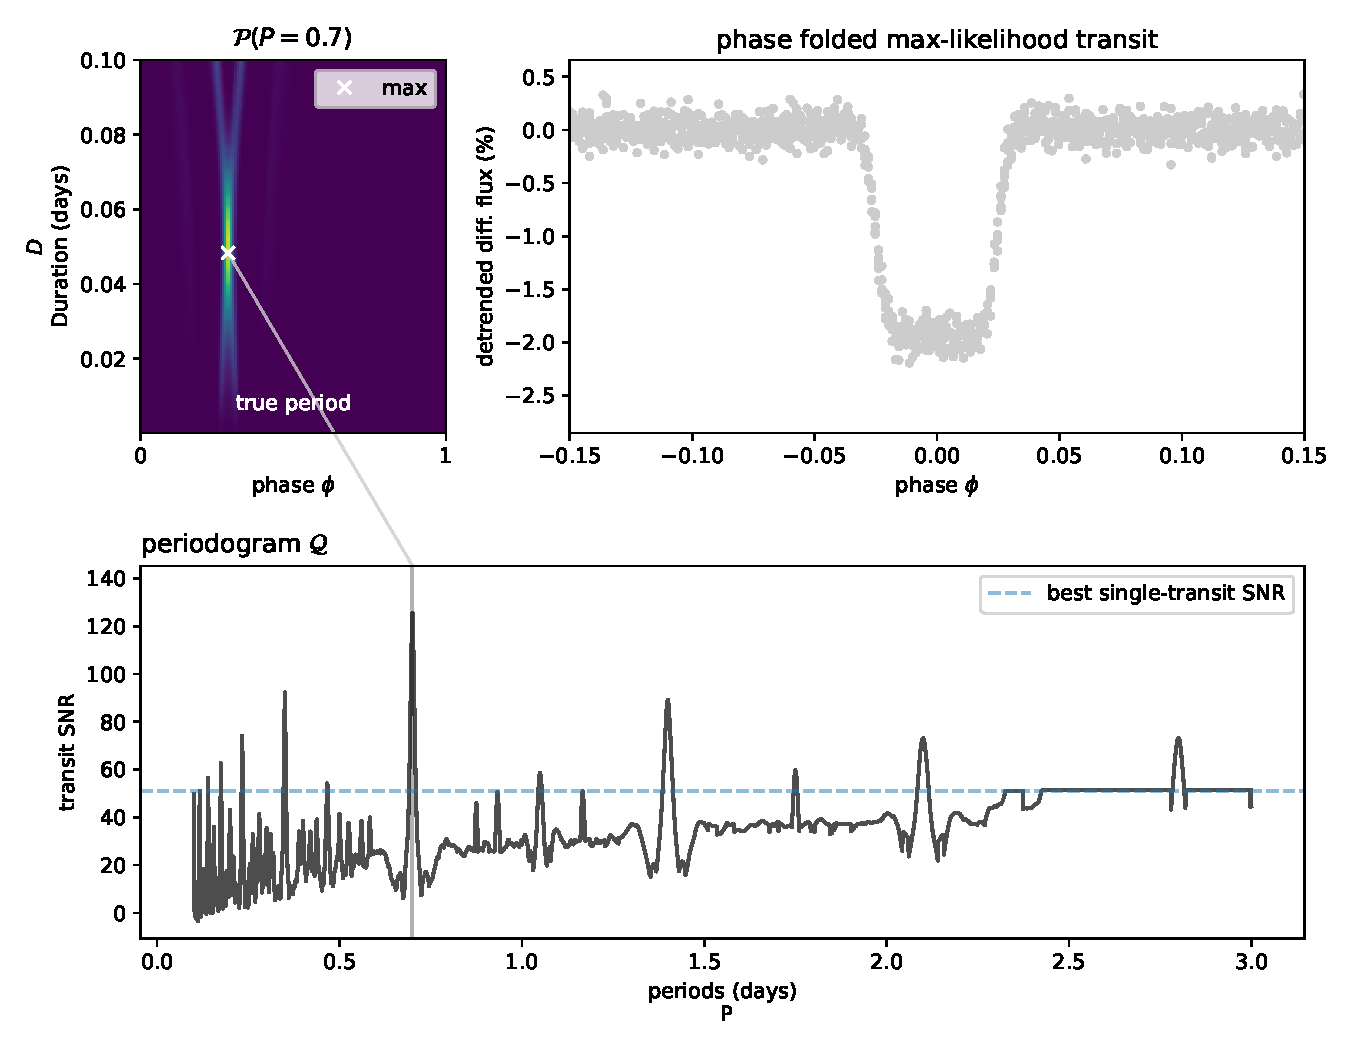
\includegraphics[width=0.8\linewidth]{principle_Q.pdf}
        \caption{For each period $P$, the joint likelihood $\mathcal{P}(P)$ is computed using \autoref{eq:result}, and the value of the maximum likelihood transit SNR retained as $\mathcal{Q}(P)$.}
        \label{fig:periodogram}
    \end{centering}
\end{figure}

\subsection{An open-source python package}
Methods presented in this paper are made accessible through the \textsf{nuance} open-source Python package, hosted on Github\footnote{\href{https://github.com/lgrcia/nuance}{https://github.com/lgrcia/nuance}} and released on the Python Package Index (PyPI)\footlink{https://pypi.org/project/nuance/}. 
\\\\
To instantiate a search, a user can start by creating a \textsf{Nuance} object with
\begin{lstlisting}[language=Python]
from nuance import Nuance

nu = Nuance(time, flux, gp=gp, X=X)
\end{lstlisting}
where \textsf{gp} is a \textsf{tinygp} Gaussian Process instance and \textsf{X} the design matrix of the linear model. \textsf{nuance} exploits the use of \textsf{tinygp}\footnote{\href{https://github.com/dfm/tinygp}{https://github.com/dfm/tinygp}}, a Python package powered by \textsf{JAX}\footnote{\href{https://github.com/google/jax}{https://github.com/google/jax}}, allowing for custom kernels to be built and highly tractable computations. We can then define a set of epochs \textsf{t0s} and durations \textsf{Ds} and run the linear search with
\begin{lstlisting}[language=Python,linewidth=\linewidth]
import numpy as np

t0s = time.copy()
# a range of 10 durations
Ds = np.linspace(0.01, 0.2, 10)
nu.linear_search(t0s, Ds)
\end{lstlisting}
Finally, the periodic search is run with
\begin{lstlisting}[language=Python]
# a wide range of periods
periods = np.linspace(0.1, 5, 2000)
search = nu.periodic_search(periods)
\end{lstlisting}
From this \texttt{search} object, the best transiting candidate parameters can be computed (\textsf{search.best}), or the $\mathcal{Q}$ periodogram retrieved (\textsf{search.Q\_snr}), together with valuable information about the transit search. The \textsf{Nuance} object also provides methods to perform transit search on light curves from multi-planetary systems, the advantage of \textsf{nuance} being that the linear search only needs to be performed ones, and reused for the search of several transiting candidates. An extensive and maintained online documentation is provided at \href{https://nuance.readthedocs.io}{\texttt{nuance.readthedocs.io}}.

\section{Control test against BLS}\label{control}

To start testing \textsf{nuance} against existing methods, a simple light curve is simulated, consisting in pure white noise with a standard deviation of $5\times 10^{-4}$ (relative flux), observed for a duration of 6 days with a cadence of 2 minutes.
In this signal, box-shaped transits are injected with periods randomly sampled from 0.3 to 2.5 days, a unique transit duration of 50 minutes, and depths randomly sampled from $2.6 \times 10^{-4}$ to $6.8 \times 10^{-4}$ (using the simple model from \cite{protopapas} presented in \autoref{app_proto} with $c=500$). By design, these injected signals have an SNR ranging from 5 to 30 (with $\sigma_r = 0$ in \autoref{eq:snr}). For each light curve, transits are searched using two different methods: \textsf{nuance}, using its implementation from the Python package described in the previous section; and \texttt{BLS}, the box-least-square algorithm \citep{bls}, using the \textsf{astropy} \textsf{BoxLeastSquares} implementation\footlink{https://docs.astropy.org/en/stable/api/astropy.timeseries.BoxLeastSquares.html}. For \nuance{}\\\\
For both methods, 3000 trial periods from 0.2 to 2.6 days are searched, with a single trial duration fixed to the unique known duration of 50 minutes. A transit signal is considered detected if the absolute difference between the injected and the recovered period is less than 0.01 day. To ease the detection criteria, transit periods recovered at half or twice the injected period (aka \textit{aliases}) are considered as being detected. For this reason, detected transit epochs are not considered. Results from this \textit{injection-recovery} procedure are shown in \autoref{fig:control}.

\begin{figure}[H]
    \begin{centering}
        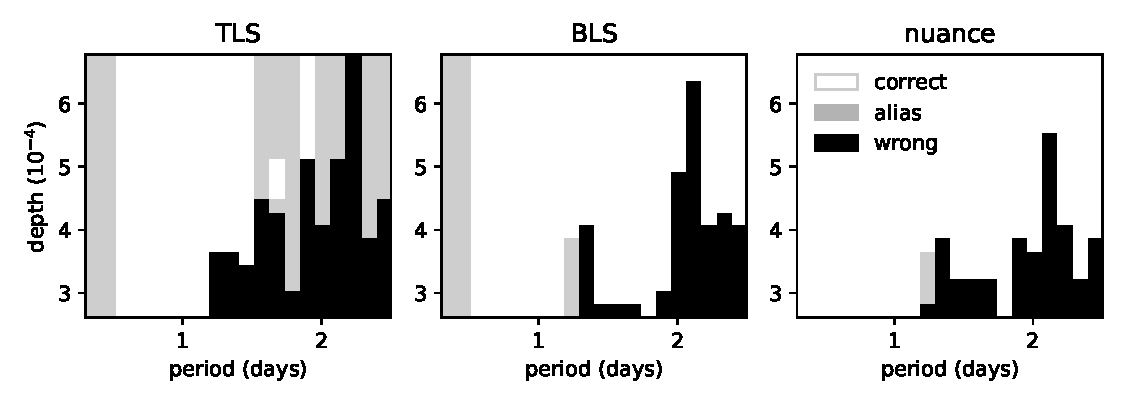
\includegraphics[width=0.85\linewidth]{../workflows/sanity/figures/control_test.pdf}
        \caption{Binned statistics of the injection-recovery of 4000 transit signals in a flat light curve with only white noise (whose characteristics are described in the main text), using \texttt{BLS} and \textsf{nuance}. The color scale indicates the recovery of transits in the corresponding (period, depth) parameters space, white for a full recovery and black for no detection.}
        \label{fig:control}
    \end{centering}
\end{figure}

These results demonstrate the qualitative match between the detection capabilities of \textsf{nuance} and \texttt{BLS} on light curves with no correlated noise. Explaining the subtle differences observed between the two methods when only white noise is present is beyond the scope of this paper, and we will assume that any differences observed in the following sections are due to the different treatments of correlated noise.

\section{\textsf{nuance} \textit{vs.} \texttt{biweight+BLS} on simulated light curves}\label{simu}
\autoref{fig:snr_detrend} shows that \textsf{nuance}'s full-fledged modeling capabilities may not always be necessary and may only be beneficial for certain noise characteristics, relative to the searched transit parameters. Here, we evaluate the performance of \textsf{nuance} in the relative parameter space $(\tau, \delta)$ described in \autoref{eq:relative_params} and see when its specific treatment of correlated noise in the transit search becomes necessary.\\\\
We compare \textsf{nuance} to the approach that involves removing stellar variability from the light curves before performing the search on a detrended dataset. Similar to \autoref{detrending_effect}, an optimal bi-weight filter implemented in the \textsf{wõtan} Python package\footlink{https://github.com/hippke/wotan} is used with a window size three times that of the injected transit duration. A transit search on the detrended light curve is then performed using the \texttt{BLS} algorithm, like in \autoref{control} using the \textsf{astropy} \textsf{BoxLeastSquares} implementation\footlink{https://docs.astropy.org/en/stable/api/astropy.timeseries.BoxLeastSquares.html}. This strategy is widely used in the community and is denoted \texttt{biweight+BLS}. In what follows, the transit detection criteria are the same as the ones used in \autoref{control}, i.e. that a transit is considered recovered if the absolute difference between the injected and recovered period is less than 0.01 days, including periods found at half or twice the injected ones (aliases) and ignoring the value of the recovered transit epoch.

%% STOPPED HERE

\subsection{Dataset}\label{sim_dataset}
The dataset consists in 4000 light curves simulated using the model fully described in \autoref{signals_simulations}. We simulate a common periodic transit added to all light curves, of period $P=1.1$ days, epoch $T_0=0.2$ days, duration $D=0.04$ days and depth $\Delta=1\%$. Each light curve consists in a 4 days observation with an exposure time of 2 minutes, leading to $N=2880$ data points with a normal error of $0.1\%$. As in \autoref{control}, only box-shaped transits are injected, using the model from \cite{protopapas} with $c=500$.
\\\\
For a given pair of $(\tau, \delta)$, we simulate stellar variability using a Gaussian Process with an SHO kernel of hyperparameters defined by \autoref{eq:relative_params} (except for $Q$, described below), computed with respect to the injected transit parameters $D$ and $\Delta$. The same kernel is used for the search with \textsf{nuance}, an optimal choice on equal footing with the optimal $3\times D$ window size of the bi-weight filter employed in the \wtls{} search. While this kernel is optimal, a comprehensive discussion on the use of non-optimal kernels is discussed in . 4000 pairs of $(\tau, \delta)$ are generated such that
\begin{equation*}
    \tau \sim \mathcal{U}(0.1, 10), \hspace{0.5cm} \delta \sim \mathcal{U}(0.1, 25) \hspace{0.5cm}\text{and}\hspace{0.5cm} Q \sim \mathcal{U}(10, 100)
\end{equation*}
where $\mathcal{U}(a, b)$ denotes a uniform distribution of lower bound $a$ and upper bound $b$.

\subsection{Results}
The results of this injection-recovery procedure are shown in \autoref{fig:simu} and highlight particularly well the benefit of \textsf{nuance} against the \wtls{} strategy on transits with relatively low depth compared to the stellar variability amplitude, and a relatively small duration compared to the stellar variability period. This empirical statement only concerns light curves with a given amount of white noise, and may vary depending on the length of the observing window or the number of transits. For this reason, quantifying for which values of $(\tau, \delta)$ \textsf{nuance} outperforms \wtls{} would only apply to this specific example. While more examples are considered in the following \autoref{real}, proper guidelines on when to use \textsf{nuance} instead of more classic detrending techniques are discussed in \autoref{when}.
\begin{figure}[H]
    \begin{centering}
        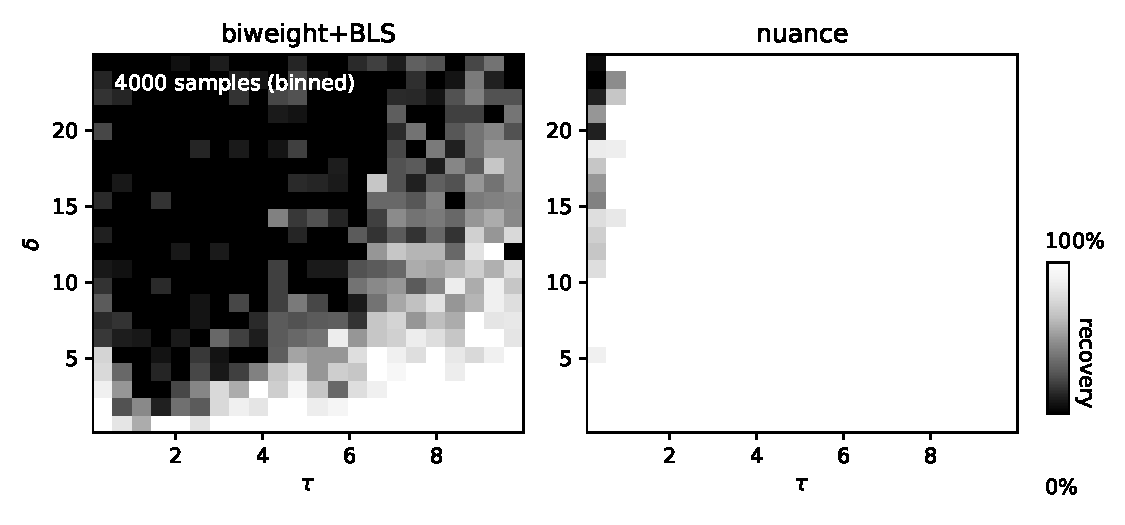
\includegraphics[width=0.85\linewidth]{../workflows/synthetic-injection-recovery/figures/synthetic_ir.pdf}
        \caption{Injection-recovery results on 4000 simulated light curves described in \autoref{sim_dataset}. The color scale represents the fraction of recovered transits, white if all injected transits are recovered in a given portion of the $(\tau, \delta)$ parameter space, black if none are recovered.}
        \label{fig:simu}
    \end{centering}
\end{figure}

\noindent This injection-recovery is done in a particularly optimal setup, on light curves not all physically realistic and using an optimal Gaussian Process kernel, hence demonstrating the performance of \textsf{nuance} only on a purely experimental basis. In the next section, we perform transits injection-recovery on real space-based light curves.


\section{Validation on TESS light curves}\label{real}

The parameter space ($\tau$, $\delta$) introduced in \autoref{detrending_effect} is very convenient from a signal processing point of view, but lacks physical reality. Very low values of $\tau$ and $\delta$ often translate into non-physical exoplanets properties as well as unrealistic stellar variability, with a strong dependence on the host star properties. \\\\
In order to assess the performance of \textsf{nuance} on real light curves, its transit recovery capabilities are rather evaluated in the planetary (period, radius) parameter space, more often encountered in the literature (e.g. Figure 12 of \citealt{Delrez2022}). In what follows, transits described by the simple model of \cite{protopapas} (see \autoref{app_proto}) are injected into light curves from the Transiting Exoplanet Survey Satellite (TESS, \citealt{tess}). We focus this proof of concept on light curves from a list of $\sim$600 M-dwarfs found to have detectable rotation signals with periods lower than one day \citep{Ramsay2020}, which lead to a parameter space justifying the use of \nuance{} (see \autoref{when}). For each of the studied target, transits are injected and recovered in the TESS 2 min cadence SPOC Simple Aperture Photometry and Pre-search Data Conditioning light curves (PDCSAP, \citealt{spoc}) on a single sector (the first being observed for each target) spanning an average of 27 days.\\\\
In the following sections, \textsf{nuance} is compared to other transit search strategies employing the \texttt{BLS} algorithm, each time after detrending the light curves with three different techniques:
\begin{itemize}
    \item \texttt{bspline+BLS} employs a B-spline\footlink{https://docs.scipy.org/doc/scipy/reference/generated/scipy.interpolate.BSpline.html} detrending, fitted using the \textsf{scipy.interpolate.splrep} function\footlink{https://docs.scipy.org/doc/scipy/reference/generated/scipy.interpolate.splrep.html}, followed by a search with the \texttt{BLS} algorithm.
    \item \texttt{biweight+BLS} employs an optimal bi-weight filter implemented in the \textsf{wõtan} Python package \citep{wotan} with an optimal window size of $3\times D$ (i.e.\, three times the transit duration), followed by a search with the \texttt{BLS} algorithm.
    \item \texttt{harmonics+BLS} employs a linear harmonic detrending, where the light curve is modeled as a Fourier series including four harmonics of the stellar rotation period found by \cite{Ramsay2020}, with coefficients found through ordinary least square. This detrending is followed by a search with the \texttt{BLS} algorithm.
\end{itemize}

\subsection{Stellar variability kernel}
A Gaussian Process kernel with a single SHO kernel is not representative of realistic stellar variability. Instead, a mixture of two SHO kernels of period $P_\star$ and $P_\star/2$ (with $P_\star$ the rotation period of the star), being representative of a wide range of stochastic variability in stellar time series from rotation to pulsations\footlink{https://celerite2.readthedocs.io/en/latest/api/python}, is adopted, with the addition of one short scale and one long term exponential term. This full rotation kernel is expressed as
\begin{equation*}
    k = k_1 + k_2 + k_3 + k_4
\end{equation*}
with
\begin{itemize}
    \item $k_1$ a SHO kernel with hyperparameters \begin{equation*}
        Q_1 = 1/2 + Q_0 + \delta Q\,, \hspace{0.5cm}
        \omega_1 = \frac{4\,\pi\,Q_1}{P\,\sqrt{4\,Q_1^2 - 1}} \hspace{0.5cm} \text{and} \hspace{0.5cm}
        S_1 = \frac{\sigma^2}{(1 + f)\,\omega_1\,Q_1}.
    \end{equation*}
    \item $k_2$ a SHO kernel with hyperparameters \begin{equation*}\begin{gathered}
        Q_2 = 1/2 + Q_0\,, \hspace{0.5cm}
        \omega_2 = 2 \omega_1 \hspace{0.5cm} \text{and} \hspace{0.5cm}
        S_2 = \frac{f\,\sigma^2}{(1 + f)\,\omega_2\,Q_2},
    \end{gathered}\end{equation*}
\end{itemize}
where $Q_0$ is the quality factor for the secondary oscillation, $\delta Q$ is the difference between the quality factors of the first and the second modes, $f$ is the fractional amplitude of the secondary mode compared to the primary and $\sigma$ is the standard deviation of the process. The kernels $k_3$ and $k_4$ are expressed as 
\begin{equation*}
        k(t, t')=\sigma^2\,\exp\left(-\frac{\vert t - t' \vert}{\ell}\right),
\end{equation*}
with $\ell$ and $\sigma$ the scale and standard deviation of the process. These are meant to model short and long timescale non-periodic correlated noise In total, the rotation kernel $k$ has 8 hyperparameters.


\subsection{Light curve cleaning}
As the described light curve model does not account for stellar flares, the light curve of each target is cleaned using an iterative sigma clipping approach. For each iteration, points 4 times above the standard deviation of the full light curve (previously subtracted by its median) are identified. Then, the 30 adjacent points on each side of the found outliers are masked. This way, large flare signals and their expected ingress and egress are masked, using a total of 3 iterations. As PDCSAP light curves often start with a ramp-like signal, the first 300 points (as well as the last 300 points) of each continuous observation are masked. Finally, each light curve is normalized by its median value. Such a cleaned light curve is shown in \autoref{fig:cleaned}.
\begin{figure}[H]
    \centering
    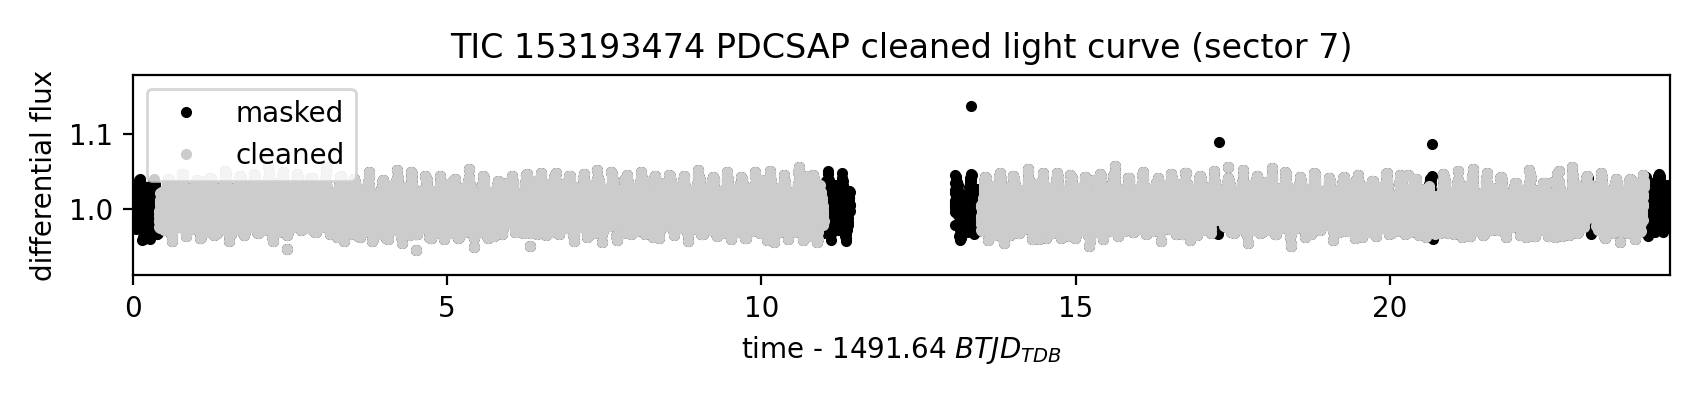
\includegraphics[width=\linewidth]{153193474_clean.png}
    \caption{Cleaned single-sector light curve of the target TIC 153193474. The light curve is normalized by its median value.}
    \label{fig:cleaned}
\end{figure}

\subsection{Injected transits}
For each target light curve, transits of planets with 10 different orbital periods combined with 10 planetary radii are individually considered, for a total of 100 periodic transits injections and recovery per target. Orbital periods $P$ are sampled on a regular grid between 0.4 and 10 days, and planetary radii $R_p$ are sampled on a regular grid designed to lead a minimum transit SNR of 4 and a maximum of 30. Using \autoref{eq:snr} with $\sigma_r = 0$, the planetary radius leading to a transit with a desired SNR $s$ is given by
\begin{equation*}
    R_p = R_{\star}\,n^{-\frac{1}{4}} \sqrt{\sigma s}\ %\sqrt[\leftroot{0}\uproot{2}4]{n}}. 
\end{equation*}
with $\sigma$ equal to the mean uncertainty estimated by the SPOC pipeline, $R_\star$ the radius of the star reported by \cite{Ramsay2020} and $n$ the number of points in transit computed using a transit duration assuming a circular orbit.

\subsection{Gaussian Process hyperparameters optimization}
The hyperparameters of the employed rotation kernel are optimized on cleaned light curves containing the injected transits, using the \textsf{scipy.optimize.minimize}\footlink{https://jax.readthedocs.io/en/latest/_autosummary/jax.scipy.optimize.minimize.html} wrapper provided by the \textsf{jaxopt} Python package, taking advantage of the \textsf{JAX} implementation of \textsf{tinygp}. As correlated noise is expected to affect the light curve uncertainty estimates performed by SPOC, the diagonal of the full covariance matrix of the data (i.e.\,their uncertainty, assuming homoscedasticity) is held free, increasing the number of optimized parameters to 9. The optimization is performed using the \textsf{BFGS} algorithm \citep{Fletcher1987}, minimizing the negative log-likelihood of the data as expressed in \autoref{eq:linear_search_ll} (without transit), i.e.\,accounting for a linear systematic model of the data in addition of stellar variability. For simplicity, and to adopt a uniform treatment for all target light curves, a design matrix $\bm{X}$ with a single constant column is adopted, such that the systematic model only consists in a single parameter corresponding to the mean value of the differential flux (expected to be close to 1) solved linearly.

\subsection{Detection criteria}
Because we also consider planets recovered with half or twice the real period, we ease the detection criteria by ignoring the match of the recovered transit epoch with the real epoch. Note that a visual vetting ensured that the found epochs were consistent with the ones injected for cases where the planet was considered detected.

\subsection{Injection-recovery studies}
\subsubsection{TIC 140212114: fast sinusoidal variability}\label{140212114}
TIC 140212114 has an effective temperature of 3595 $\pm$ 157 K\footlink{https://exofop.ipac.caltech.edu/tess/target.php?id=140212114} (M1.5-type star, \citealt{Rajpurohit2013}) with a rotation period of 0.14 days \citep{Ramsay2020}. For each technique, the left plot of \autoref{fig:140212114} shows a portion of TIC 140212114 cleaned light curve with an injected transit signal (hardly distinguishable due to correlated noise of the light curve compared to the transit depth). On these plots the black lines correspond to the trends computed for this injected light curve subtracted from it before being searched for transits. This detrending only applies to techniques other than \textsf{nuance}, where instead the black line corresponds to the mean of the Gaussian Process model. For each technique, the right plot of \autoref{fig:140212114} shows the results of the transit search for each of the 10 $\times$ 10 injected light curves, reported in the planetary (period, radius) parameter space. A black square denotes that the transit signal has not been detected, a gray square denotes a signal detected at an alias period ($P/2$ or $2P$), and a white square denotes a transit signal detected with the correct period. On the right plots of \autoref{fig:140212114}, secondary axes show the values of the injected transits in the $(\tau, \delta)$ relative parameter space.\\\\
Results from \autoref{fig:140212114} are discussed in \autoref{tess_results}.

\begin{figure}[H]
    \begin{centering}
        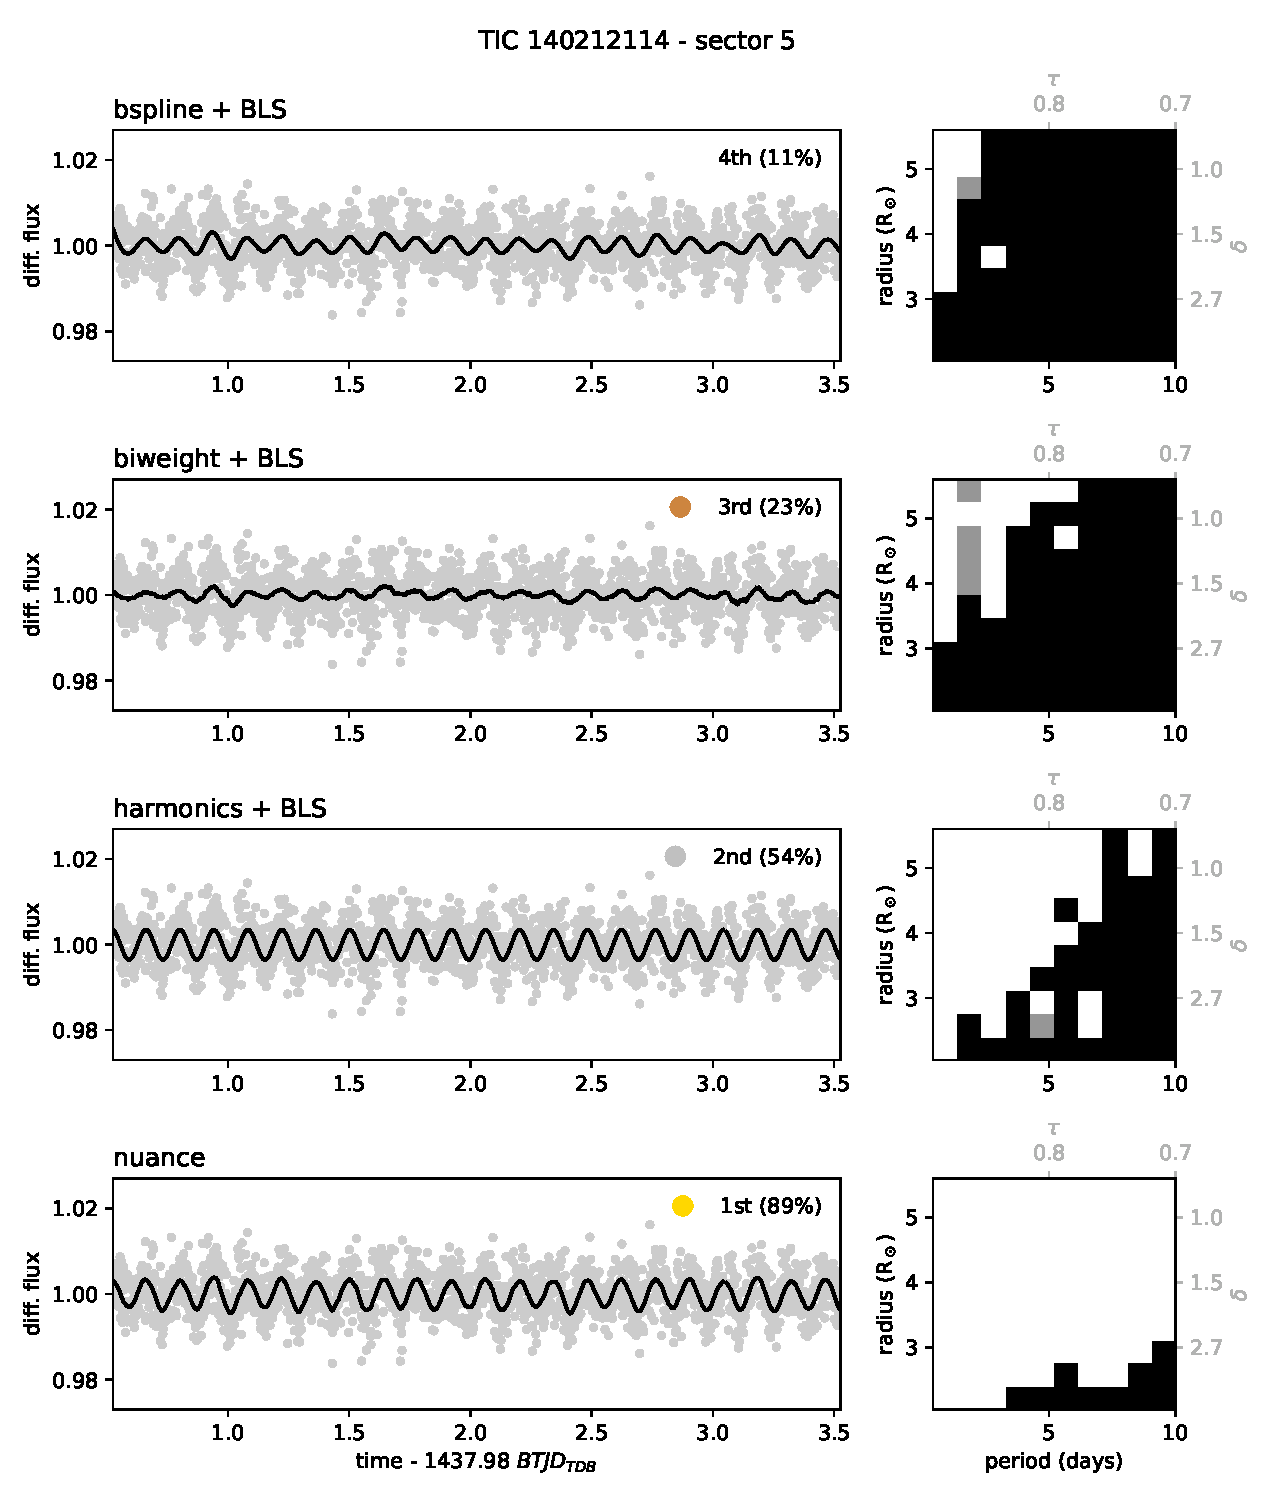
\includegraphics[width=0.8\linewidth]{140212114.pdf}
        \caption{Results of the transits injection-recovery on TIC 140212114 single-sector light curve. Left: cleaned light curve with computed trend overplotted in black (except for \textsf{nuance} where it corresponds to the mean of the Gaussian Process model). Right: Results of the transit search where a black square denotes a transit signal not detected, gray a signal detected at an alias period ($P/2$ or $2P$), and  white a signal detected with the correct period. On the right plots, secondary axes show the $(\tau, \delta)$ relative parameter space. For each method, the upper right legend on the left plot indicates its ranking based on the percent of recovered transit signals (where a transit with an aliased period counts as being detected). The \texttt{harmonics+TLS} method is the best after \textsf{nuance}, but with 35\% less transits detected in total. 
        }
        \label{fig:140212114}
    \end{centering}
\end{figure}

\subsubsection*{TIC 452793374: high-amplitude red noise}
TIC 452793374 has an effective temperature of 3377 $\pm$ 157 K\footlink{https://exofop.ipac.caltech.edu/tess/target.php?id=452793374} (M2.5-type star, \citealt{Rajpurohit2013}) with a rotation period of 0.33 days \citep{Ramsay2020}. Injection-recovery results are shown in \autoref{fig:452793374} and discussed in \autoref{tess_results}.

\subsubsection*{TIC 153193474: non-sinusoidal variability}
TIC 153193474 has an effective temperature of 3351 $\pm$ 157 K\footlink{https://exofop.ipac.caltech.edu/tess/target.php?id=27734884} (M2.5-type star, \citealt{Rajpurohit2013}) with a rotation period of 0.11 days \citep{Ramsay2020}. Injection-recovery results are shown in \autoref{fig:153193474} and discussed in \autoref{tess_results}.

\subsubsection*{TIC 306331621: slow sinusoidal variability}
TIC 306331621 has an effective temperature of 3067 $\pm$ 157 K\footlink{https://exofop.ipac.caltech.edu/tess/target.php?id=306331621} (M5-type star, \citealt{Rajpurohit2013}) with a rotation period of 1.00 days \citep{Ramsay2020}. It was chosen for its relatively slow rotation (compared to the three other targets) and higher white noise compared to the amplitude of its variability. Injection-recovery results are shown in \autoref{fig:306331621} and discussed in \autoref{tess_results}.

\subsection{Results}\label{tess_results}

From the injection-recovery conducted on TIC 140212114, TIC 452793374, TIC 153193474 and TIC 306331621, it can be concluded that searching for transits directly with \textsf{nuance} offers a clear advantage over any of the presented detrending methods combined with \texttt{BLS}. While not fully described in this dissertation, injection-recovery on additional targets lead to a similar conclusion.\\\\
Targets with light curves featuring stable sinusoidal stellar variability, i.e.\,with a high quality factor $Q$ (see the SHO kernel), are the ones that benefit less from \textsf{nuance}, as a set of harmonic signals can be combined linearly to robustly model and detrend the periodic signal. In the cases of TIC 452793374 and TIC 306331621, an additional $\sim$6\% of planets are detected by \textsf{nuance} over the probed planetary (period, radius) parameter space. From these two examples, it cannot be concluded if this difference is solely due to the difference observed between \textsf{nuance} and \texttt{BLS} in \autoref{control} . While red noise was properly detrended by a bi-weight filter in the case of TIC 452793374, additional tests must be done to show that \textsf{nuance} clearly outperforms this method when any red noise is present in the light curve (as partially observed in \autoref{simu}).
\\\\
Finally, targets with non-sinusoidal or short scale variability are the ones that benefit the most from \textsf{nuance}, as no other method is able to robustly detrend their light curves  without removing transit signals. This is well illustrated by the study of TIC 140212114 (\autoref{fig:140212114}) and TIC 153193474 (\autoref{fig:153193474}).
\begin{figure}[H]
    \begin{centering}
        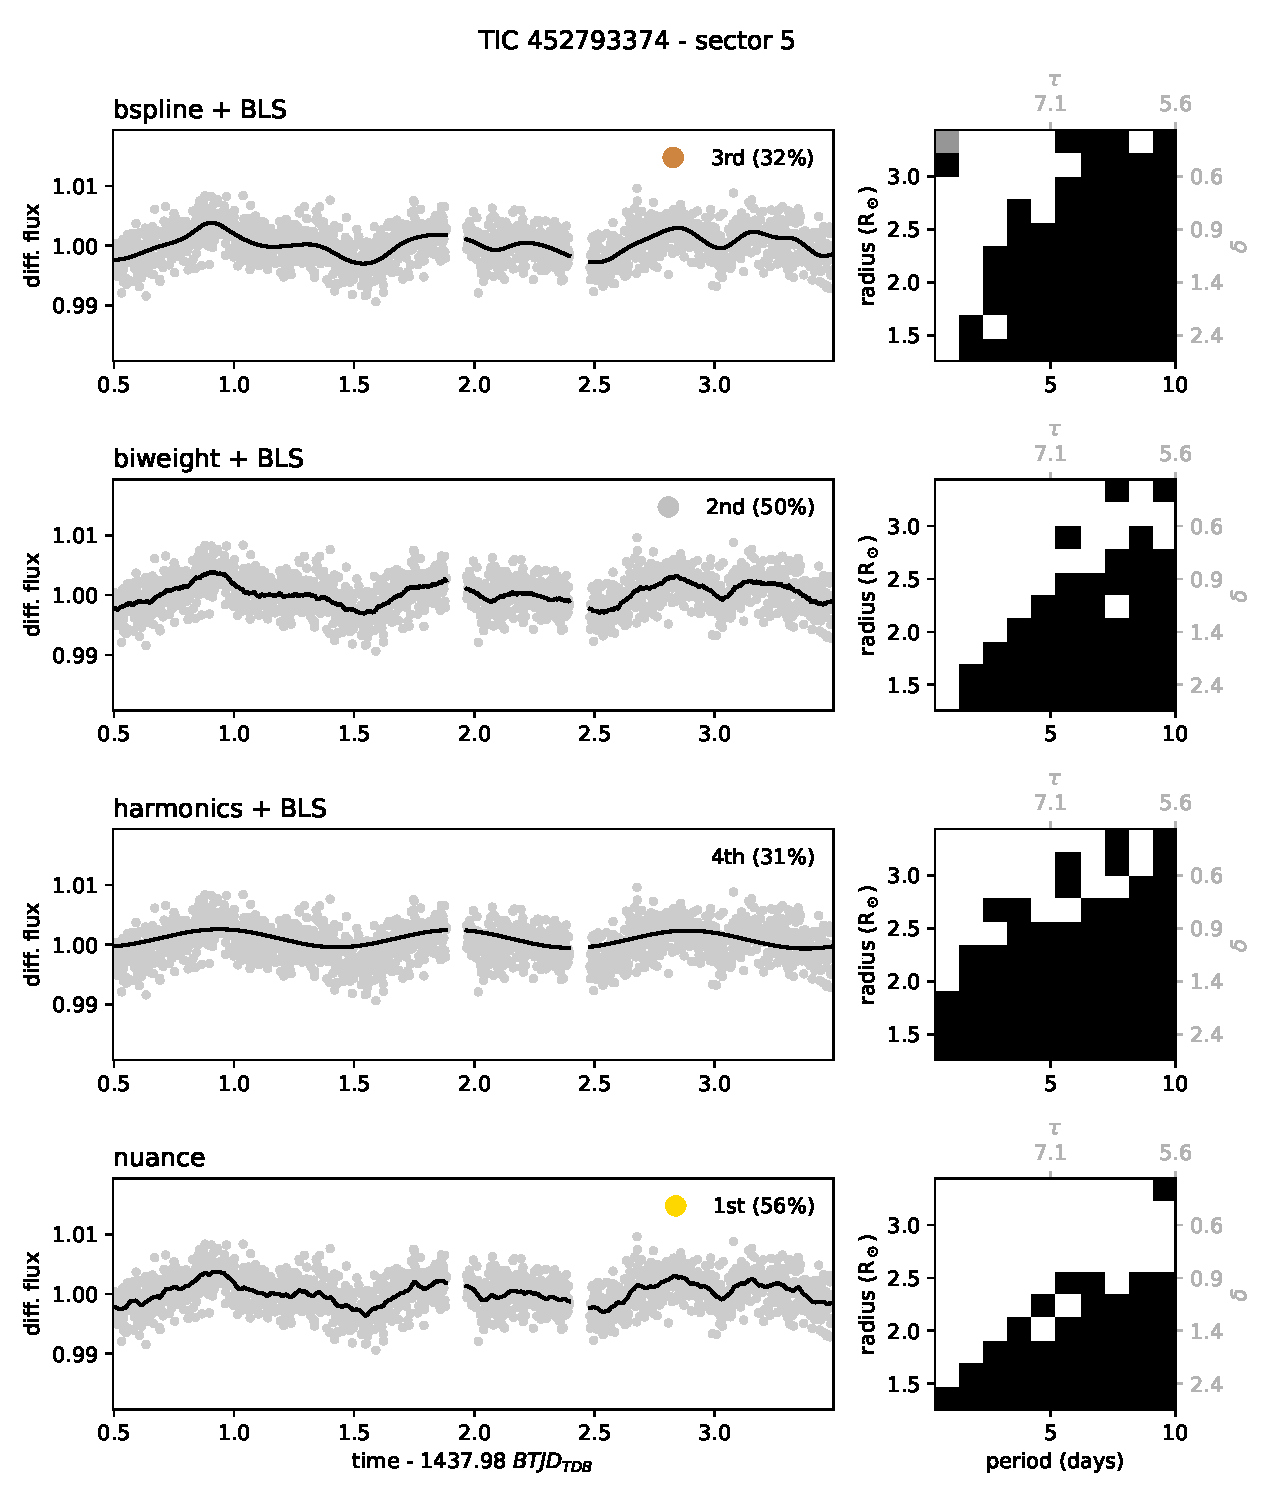
\includegraphics[width=\linewidth]{452793374.pdf}
        \caption{Results of the transits injection-recovery on TIC 452793374 single-sector light curve. See \autoref{140212114} and legend of \autoref{fig:140212114} for a detailed description of this figure. The \texttt{biweight+TLS} method is the best after \textsf{nuance}, with 6\% less transits detected in total that could be due to the sole difference between \textsf{nuance} and \texttt{BLS} discussed in \autoref{control}. It indicates that a more flexible filter is necessary for this light curve with significantly higher red noise, making \textsf{nuance} not necessary.
        }
        \label{fig:452793374}
    \end{centering}
\end{figure}

\begin{figure}[H]
    \begin{centering}
        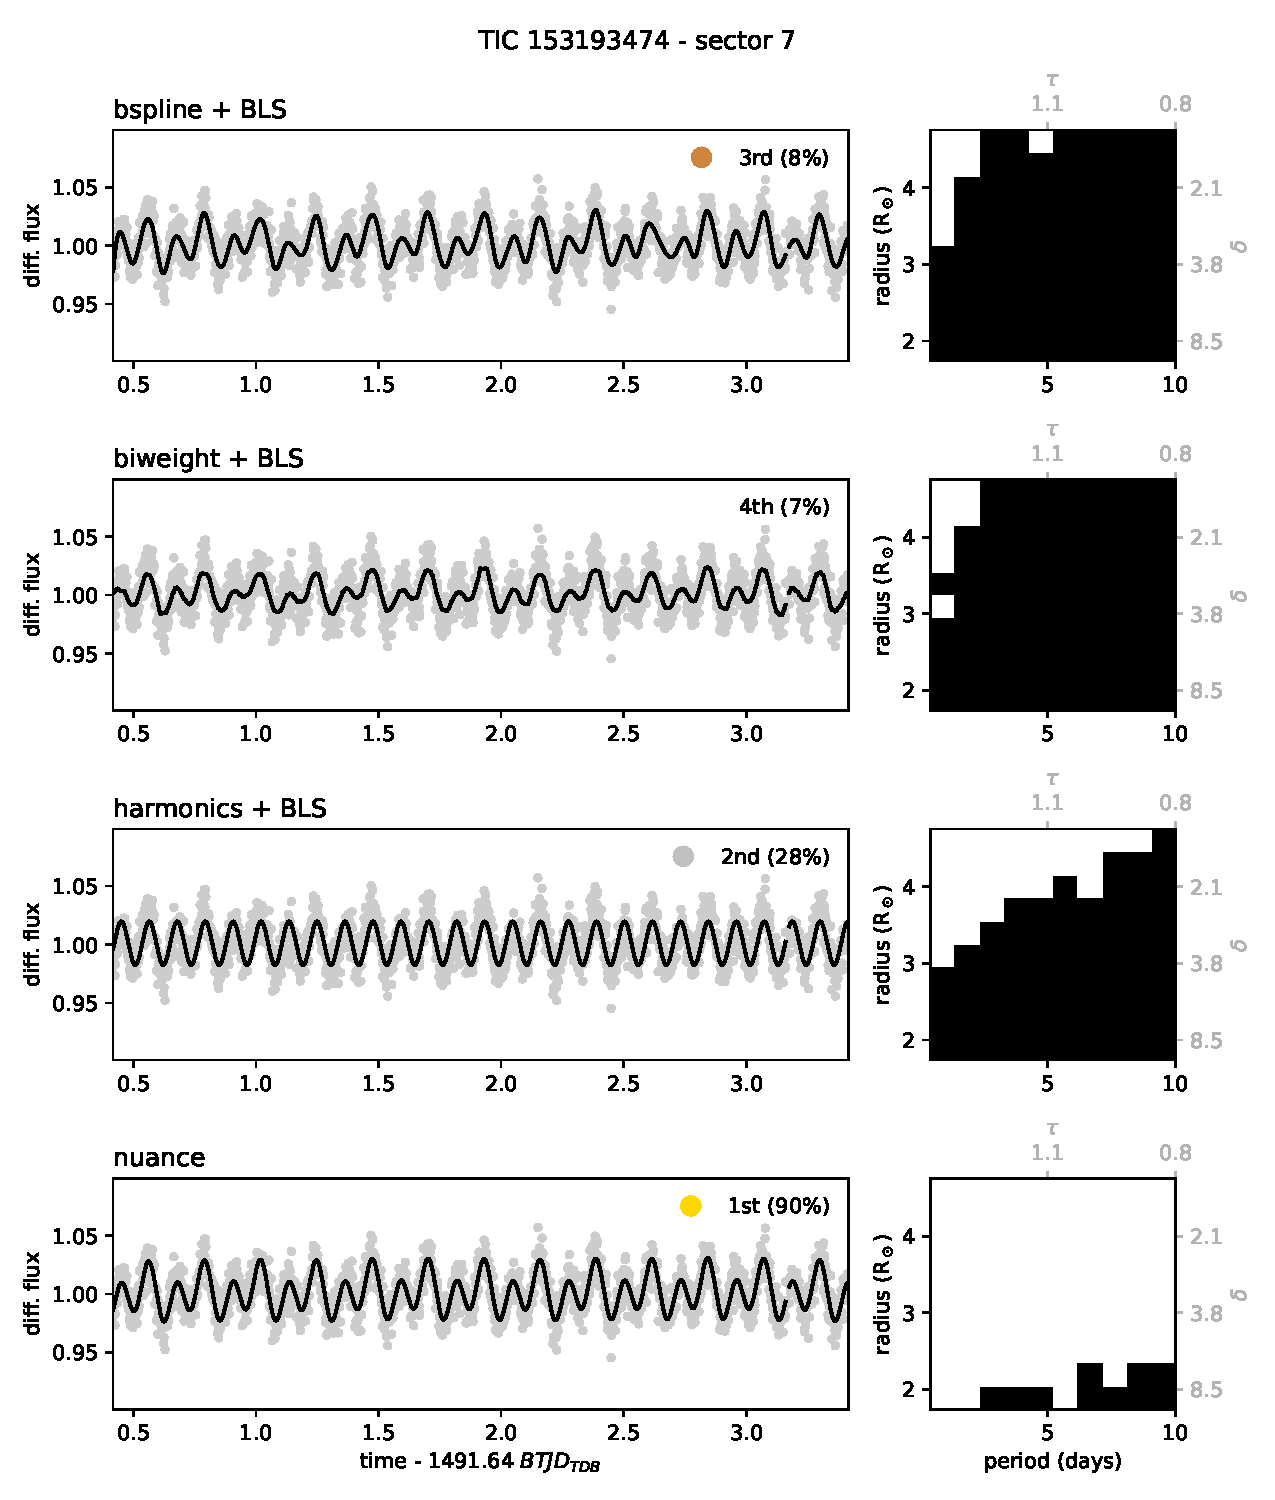
\includegraphics[width=\linewidth]{153193474.pdf}
        \caption{Results of the transits injection-recovery on TIC 153193474 single-sector light curve. See \autoref{140212114} and legend of \autoref{fig:140212114} for a detailed description of this figure. The \texttt{harmonics+TLS} method is the best after \textsf{nuance}, with 62\% less transits detected in total, indicating that all presented methods are unable to detrend without removing many of the injected transit signals (which is not surprising when considering the trend being built, except in the case of \texttt{bspline+TLS}, but being apparently too flexible).}
        \label{fig:153193474}
    \end{centering}
\end{figure}

\begin{figure}[H]
    \begin{centering}
        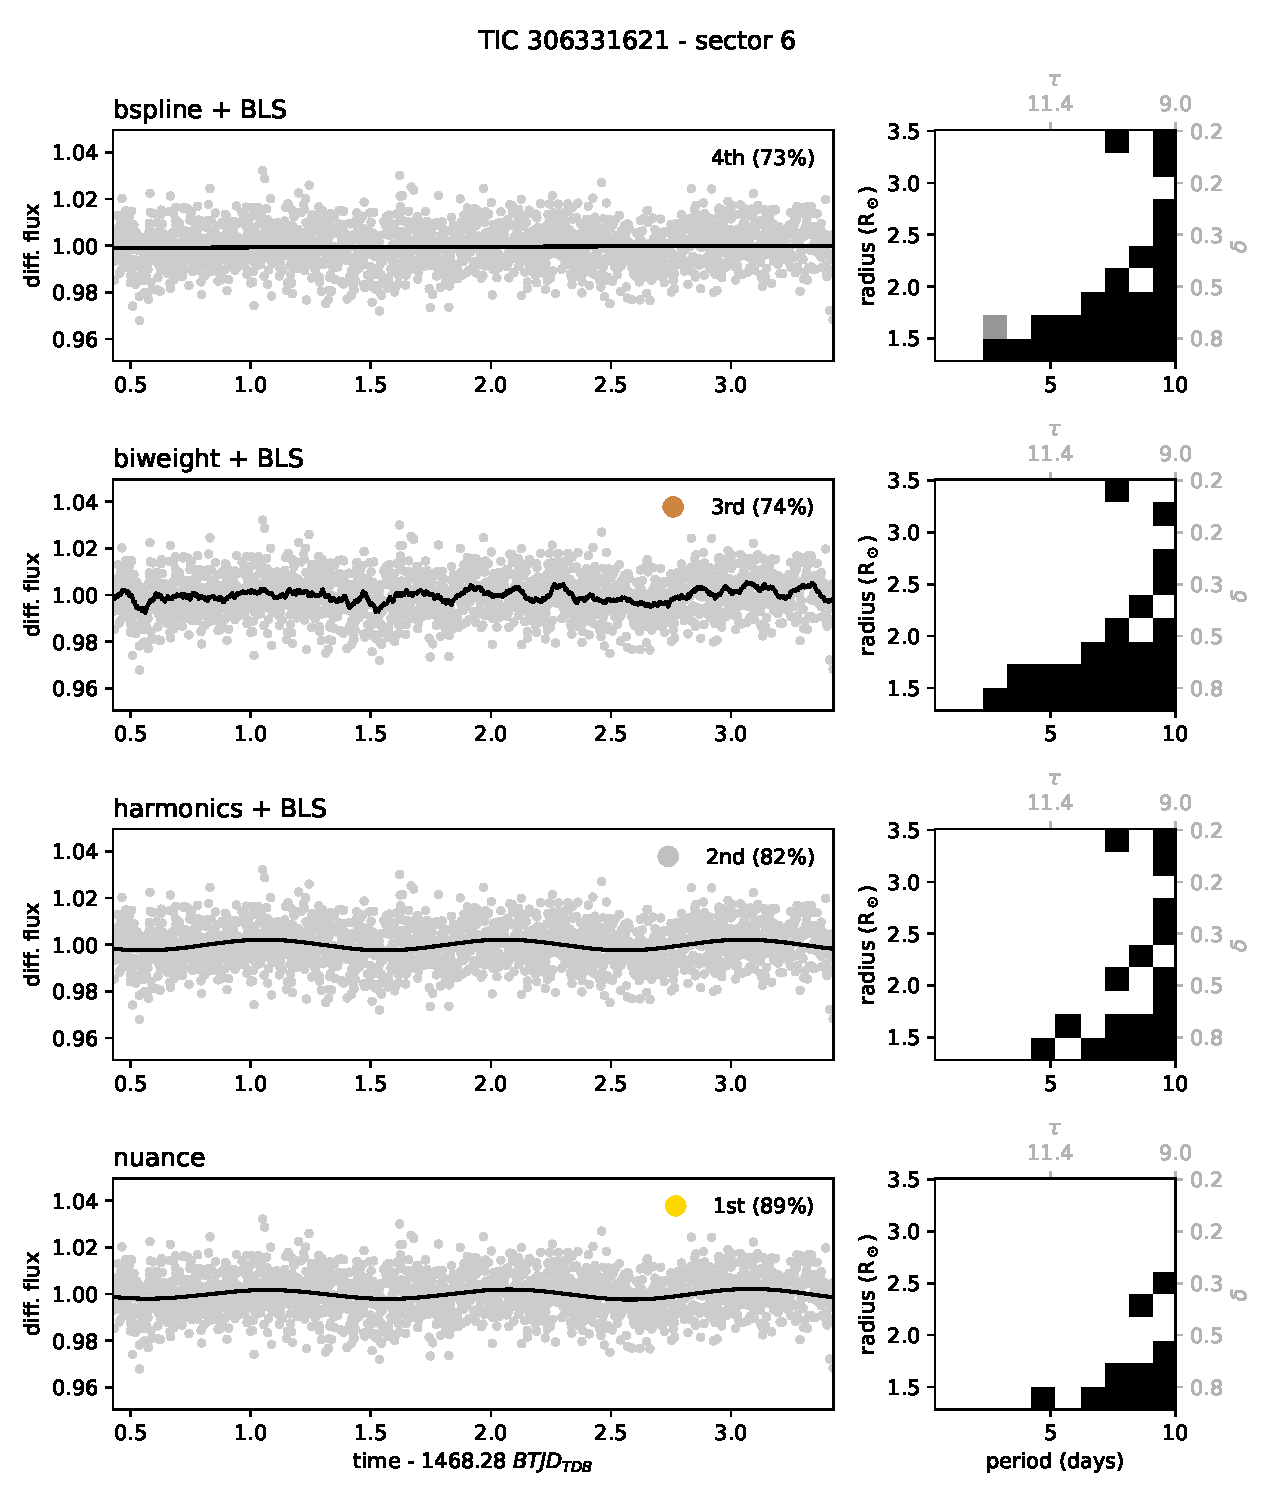
\includegraphics[width=\linewidth]{306331621.pdf}
        \caption{Results of the transits injection-recovery on TIC 306331621 single-sector light curve. See \autoref{140212114} and legend of \autoref{fig:140212114} for a detailed description of this figure. The \texttt{harmonics+TLS} method is the best after \textsf{nuance}, with 7\% less transits detected in total that could, again, be due to the sole difference between \textsf{nuance} and \texttt{BLS} discussed in \autoref{control}.}
        \label{fig:306331621}
    \end{centering}
\end{figure}

\newpage
\section{Discussion}\label{perf}

The results from \autoref{real} show that \textsf{nuance} always outperforms other methods when searching for transit signals in light curves containing correlated noise. While performances with other methods can be very comparable, \textsf{nuance} alleviates the need to choose for a specific detrending technique and rather exploit the complete modeling of the light curve using a physically interpretable Gaussian Process.\\\\
In few cases, \textsf{nuance} offers a clear advantage in comparison with other methods, in particular for low SNR transit signals in light curves containing fast or non-sinusoidal stellar variability. In these cases, \textsf{nuance} is able to robustly detect transits, and provide a unique option in comparison with techniques that likely degrade the searched signals through detrending.

\subsection*{Processing time}
As of June 2023, \textsf{nuance} is very much a work in progress and a full assessment of its performances is still ongoing. \autoref{fig:blsvsnuance} is a preliminary study of the computational cost of \textsf{nuance} against \texttt{BLS}. For reasons described in the next section, the linear search is first considered separately from the periodic search.

\begin{figure}[H]
    \begin{centering}
        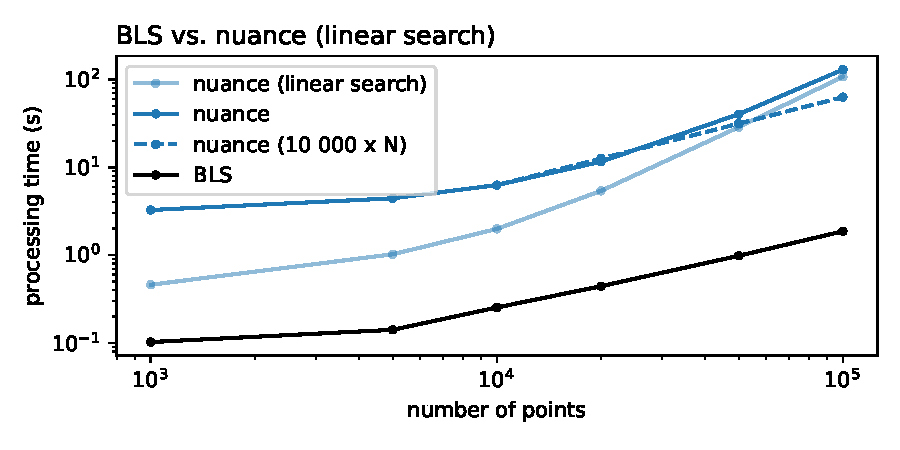
\includegraphics[width=0.8\linewidth]{nuance_vs_bls_time.pdf}
        \caption{Preliminary study of \textsf{nuance} processing time against \texttt{BLS}. The lighter blue curve shows the performance of \textsf{nuance} when applied to chunks of 10 000 points continuous observations, instead of considering these observations all together (the only option when using \texttt{BLS}).}
        \label{fig:blsvsnuance}
    \end{centering}
\end{figure}

\noindent In \autoref{fig:blsvsnuance}, the processing time of the linear search from \textsf{nuance} is recorded against the number of points in the light curve. One advantage of \textsf{nuance} is that the linear search can be performed separately on different continuous observations, and then combined in the periodic search. Hence, if searching for transits in separate observations with similar durations (such as different TESS sectors or different ground-based nightly observations), the computational cost of \textsf{nuance} grows linearly with the number of observations. Such a parallel cannot be made with \texttt{BLS}, as the algorithm considers all observations as a single one. This way, after assuming that 10 000 points observations can be combined into the periodic search (roughly corresponding to the number of data points in continuous TESS observations for example), \textsf{nuance} will constantly perform a single order of magnitude slower than \texttt{BLS}, only considering the linear search. For this reason, \textsf{nuance} must not be employed in the general case, but rather used when light curves contain correlated noise with characteristics described in this chapter. Proper guidelines and metrics to assess the presence of such noise, which would indicate if \textsf{nuance} is required, are currently being developed.\\\\
For reference, the complete search (including the periodic search) of a single TESS sector for TIC 140212114 (15992 points partly shown in  \autoref{fig:140212114}) took a total of 30 seconds, executed on a 10 core Apple M1 Pro chip. The latter processing time would grow linearly with the number of sectors being processed.

\subsection*{Periodic search}

The periodic search of \textsf{nuance} can be done separately from the linear search. For a given light curve, a single linear search can be performed then masked and combined iteratively to search for multiple transiting exoplanets. Hence, \autoref{fig:blsvsnuance} only shows the processing time of the linear search, assuming that a single planet is searched for. As of June 2023, the periodic search in the current implementation of \textsf{nuance} is the least optimized part. But recent developments indicate that the periodic search can be performed in a time equal to the complete processing time of the \texttt{BLS} algorithm. Hence, as the \texttt{BLS} algorithm grows linearly with the number of planets being searched (because reran every time on masked light curves), the increased computing time for \textsf{nuance} would be equal, bridging the gap between the computing time of  \texttt{BLS} and \textsf{nuance} when searching for multiplanetary transiting systems.

\subsection*{Design matrix}

In this chapter, starting from \autoref{detrending_effect}, it was assumed that systematic signals (as opposed to astrophysical signals) were completely corrected for without affecting the searched transit signals. For this reason, all analyses in this chapter were done with a single column design matrix $\bm{X}$, corresponding to the mean, constant, differential flux (ideally 1) of a light curve. In practice, \textsf{nuance} has been developed to linearly model systematic signals through more complex design matrices, in addition with its capability to model correlated noise while searching for transits. This aspect is completely unexploited in the previous comparisons, and would require to search for transits in completely raw light curves, which comes with few challenges. Given a light curve, this approach involves choosing a design matrix containing specific explanatory measurements, hence requiring a proper model comparison. In addition, large design matrices are expected to increase \textsf{nuance} processing time, something that needs to be accounted for in its performance assessment.\\\\
Used in the context of the SPECULOOS survey, \textsf{nuance} is currently being tested on light curves containing systematic signals that can be modeled linearly using polynomials of common explanatory variables (such as airmass, background flux, pointing error or PSF full-width at half-maximum). On light curves spanning only few hours, with less than a thousand photometric measurements, the use of a linear model to detrend the light curve ignoring the presence of transits is highly susceptible to remove the signals of interest, giving a clear advantage to a full-fledge method like \textsf{nuance}. The same applies for filter-based detrending algorithms. Proving the later empirical statement is out of the scope of this chapter and will be treated in a following publication. However, \textsf{nuance} might be particularly well suited to search for transits in ground-based observations, where the detrending of sparse observations is believed to remove the lowest SNR transit signals.\\\\
Overall, \textsf{nuance} is a powerful tool to search for transits in light curves containing systematic signals and correlated noise, characteristic of late M-dwarfs light curves. Due to several advances in computational methods, as well as its analytical formalism, \textsf{nuance}  remains highly tractable, and may already be applied to space-based continuous observations. \textsf{nuance} is currently being tested on sparse observations, offering a unique tool to search for transiting exoplanet in the light curves of SPECULOOS and other ground-based surveys. 

\subsection{When to use it?}\label{when}

% APPENDIX

\newpage
\appendix
\section{Light curves simulations}\label{signals_simulations}

In order to study the effect of correlated noise on transit search, this paper relies on transit light curve simulations including realistic effects of stellar variability and instrumental signals. The following describes how such signals are modeled.
\begin{figure}[H]
    \begin{centering}
        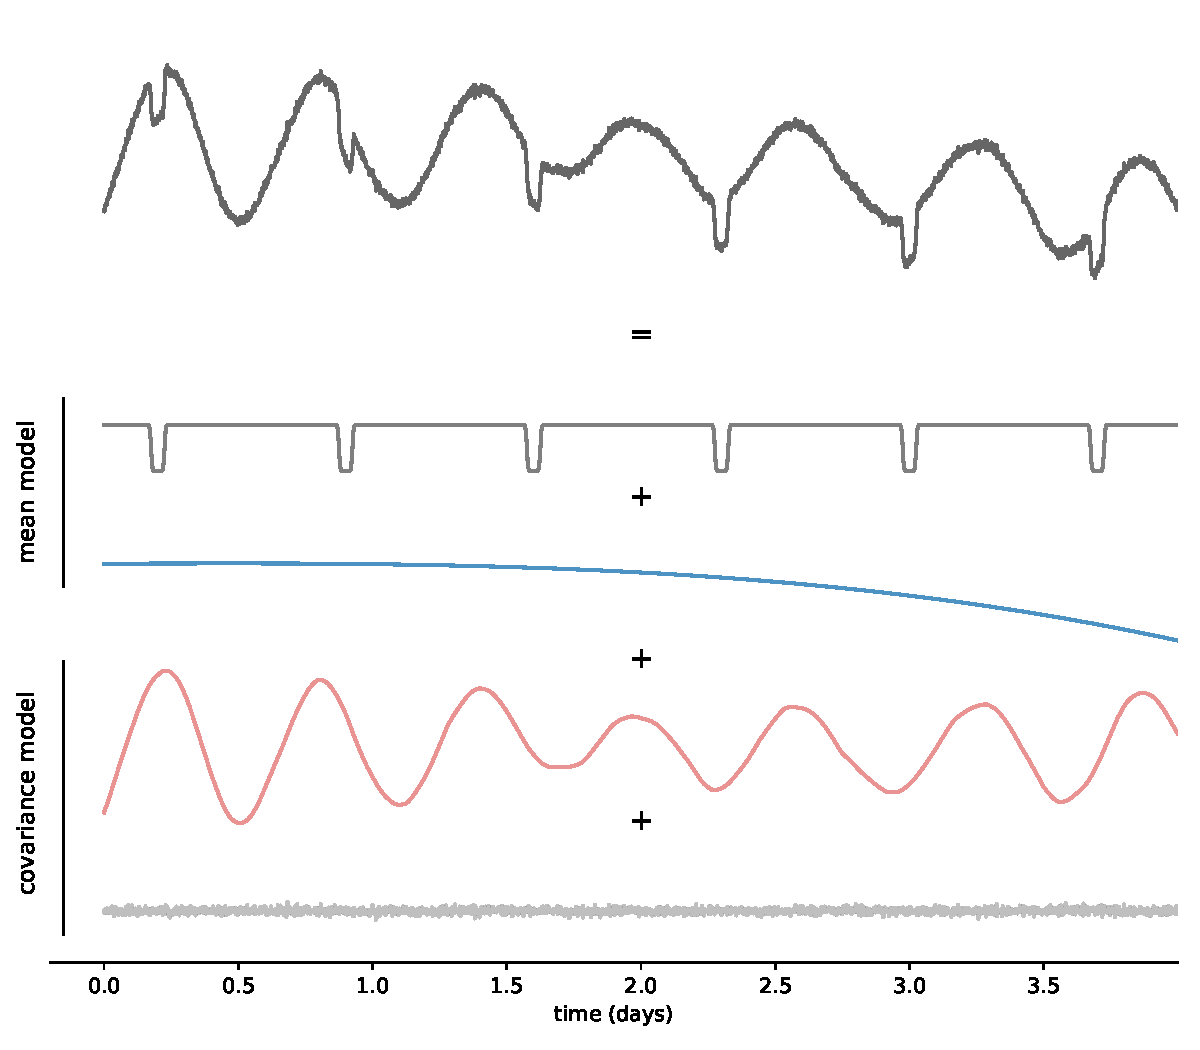
\includegraphics[width=0.75\linewidth]{principle_dataset_decomposed.pdf}
        \caption{Example dataset sampled at $N=2880$ times corresponding to an observation of 4 days with an exposure time of 2 minutes. The mean of this signal consists in a periodic transit signal of period $P=0.7$ days, duration $D=0.05$ days and depth of 2\% ($\mathcal{T}$ in gray) plus instrumental signals ($\mathcal{S}$ in blue). Correlated noise in the form of stellar variability is simulated by modeling the covariance matrix of the signal with a Gaussian process ($\mathcal{V}$ in red) including a diagonal variance of $0.001^2$ corresponding to white noise ($\epsilon$ in light grey). This simulated signal is not intended to be physically realistic.}
        \label{fig:app_principle_dataset}
    \end{centering}
\end{figure}
\noindent Let $f$ be the simulated flux of a star sampled and arranged in the vector $\bm{f}$ associated to the vector of times $\bm{t}$, such that
\begin{equation*}
    \bm{f} \sim \mathcal{N}(\bm{\mu}, \bm{C}),
\end{equation*}
i.e. that $\bm{f}$ is drawn from a Gaussian process of mean $\bm{\mu}$ and covariance matrix $\bm{C}$. In this equation, $\bm{\mu}$ is such that its $i$-th element is defined by  $\mu_i = \mathcal{T}(t_i) + \mathcal{S}(t_i)$ where $t_i$ is the $i$-th time of observation, $\mathcal{T}$ is a periodic transit function and $\mathcal{S}$ a function describing the instrumental part of the signal (both described below). The covariance matrix $\bm{C}$ is built such that $C_{i, j} = k(t_i, t_j)$ where $k$ is a covariance function (or \textit{kernel}) accounting for correlated noise in the form of stellar variability (with added white noise). An example of such signal is simulated and shown in \autoref{fig:app_principle_dataset}.

\subsection{Transit signal $\mathcal{T}$}\label{app_proto}
The periodic transit signal $\mathcal{T}$ is simulated using the simple model described in \cite{protopapas}, where a transit of period $P$, epoch $T_0$, duration $D$ and unitary depth observed at time $t$ is given by
\begin{equation}\label{eq:protopapas}
    \begin{gathered}
        \mathcal{T}_c(t, P, T_0, D) = \frac{1}{2}\tanh\left(c\left[\theta - \frac{1}{2}\right]\right) - \frac{1}{2}\tanh\left(c\left[\theta + \frac{1}{2}\right]\right), \\
        \text{with}\quad\theta = \frac{P}{\pi  D}\sin\left(\frac{\pi(t-T_0)}{P}\right),
    \end{gathered}
\end{equation}
where the dimensionless parameter $c$ controls the roundness of the transit depth ($c\gg1$ corresponding to a box-shaped transit as shown in \autoref{fig:protopapas}). This analytical model is fully empirical but easily differentiable.
\begin{figure}[H]
    \begin{centering}
        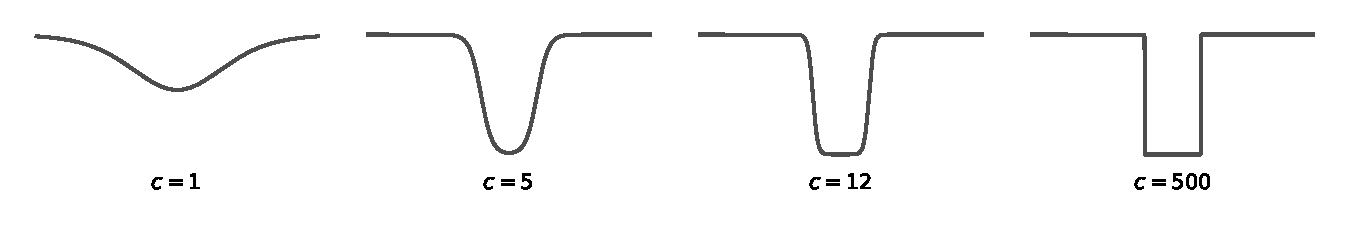
\includegraphics[width=\linewidth]{protopapas.pdf}
        \caption{Simulations of a single transit signal (\autoref{eq:protopapas}) shown for different values of $c$.}
        \label{fig:protopapas}
    \end{centering}
\end{figure}
\noindent In this paper, unless specified, all transits are simulated with $c=12$, a value arbitrarily chosen that can be fined-tuned in real applications using the limb-darkening coefficients of a given star. The periodic transit signal $\mathcal{T}$ seen in \autoref{fig:app_principle_dataset} corresponds to $\mathcal{T} = 0.02 \times \mathcal{T}_{c=12}(\bm{t}, P=0.7, T_0=0.2, D=0.05)$, all parameters in unit of days.

\subsection{Instrumental signals $\mathcal{S}$}
Instrumental signals are simulated as a linear model of $M$ explanatory variables arranged in the $(N\times M)$ design matrix $\bm{X}$. Hence,
$$
    \mathcal{S} = \bm{X w},
$$
where the vector $\bm{w}$ contains the linear coefficients of the model. The simulated flux shown in \autoref{fig:app_principle_dataset} contains a linear model where the $M=4$ columns of the design matrix $\bm{X}$ are given by $\bm{X}_{i} = \bm{t}^i$ (i.e. $\bm{X}$ is the Vandermonde matrix order $3$ of time $t$) and $\bm{w} = [1.0\quad0.0005\quad\text{-}0.0002\quad\text{-}0.0005].$

\subsection{Stellar variability $\nu$}\label{app_gp}
As this chapter focuses on stellar variability and its effect on transit detection, We employ a simple physically-motivated Gaussian Process kernel, describing stellar variability through the covariance of a stochastically-driven damped harmonic oscillator (SHO, \citealt{celerite, celerite2}) taking the form 
\begin{equation}
    \begin{gathered}
        k(\tau) = \sigma^2\,\exp\left(-\frac{\omega\,\tau}{2\,Q}\right)
        \left\{\begin{array}{ll}
            1 + \omega\,\tau & \mbox{for } Q = 1/2 \\
            \cosh(f\,\omega\,\tau/2\,Q) + \sinh(f\,\omega\,\tau/2\,Q)/f
                & \mbox{for } Q < 1/2 \\
            \cos(g\,\omega\,\tau/2\,Q) + \sin(g\,\omega\,\tau/2\,Q)/g
                & \mbox{for } Q > 1/2
        \end{array}\right. \\
        \text{where}\quad \tau = |t_i - t_j|\text{,}\quad f = \sqrt{1 - 4\,Q^2} \quad \text{and}\quad g = \sqrt{4\,Q^2 - 1}
    \end{gathered}
\end{equation}
where $Q$ is the quality factor of the oscillator, $\omega$ its pulsation and $\sigma$ the amplitude of the kernel function. Gaussian Process computations in this paper use the implementation from \texttt{tinygp}\footnote{\href{https://github.com/dfm/tinygp}{https://github.com/dfm/tinygp}}, a Python package exposing the quasi-separable kernels from \cite{celerite2} and powered by \texttt{JAX}\footnote{\href{https://github.com/google/jax}{https://github.com/google/jax}}. The stellar variability signal in \autoref{fig:app_principle_dataset} has been sampled from a Gaussian Process with an SHO kernel of parameters $\omega = \pi/6D$ (i.e. a period equal to 12 times the duration $D$ of the simulated transit), $Q=45$ and $\sigma=0.02$, the depth of the simulated transit. An extra term $\sigma_f^2=0.001^2$ is added to the diagonal of the covariance matrix, corresponding to the variance of the simulated measurement $f$ and leading to the white noise observed in \autoref{fig:app_principle_dataset}.

\section{Proof for the periodic search expression}\label{proof}

\newcommand{\sumTk}{i\neq k}
From the linear search presented in \autoref{linear_search}, we retain and index by $k$ the parameters of the $K$ individual transits whose epochs $\{T_k\}_k$ are compatible with a periodic signal of period $P$ and epoch $T_0$. From the likelihoods of these transits (computed in \autoref{linear_search}), we want an expression for
\begin{equation*}
    p(\bm{f} \vert P, T_0 ,D, \Delta) = \prod_{k\in\mathbb{T}} p(\bm{f} \vert T_k, D, \Delta),
\end{equation*}
i.e., given a depth $D$, the likelihood of the data given a periodic transit signal of period $P$, epoch $T_0$ and a common depth $\Delta$. Since only $\{p(\bm{f} \vert T_k, D, \Delta_k)\}_{k}$ is known (i.e. transits with different depths), we decompose
\begin{equation}\label{eq:non_part_of_per}
    p(\bm{f} \vert T_k, D, \Delta) = \int p(\bm{f} \vert T_k, D, \tilde\Delta)p(\tilde\Delta | \Delta)\, d\tilde\Delta,
\end{equation}
where $p(\bm{f} \vert T_k, D, \tilde\Delta)$ is the probability of the $k$-th transit to have a depth $\tilde\Delta$ and $p(\tilde\Delta | \Delta)$ the probability to observe the depth $\tilde\Delta$ knowing the existence of a common depth $\Delta$. In other words, \autoref{eq:non_part_of_per} involves the likelihood of the non-periodic transit $k$ to be part of a periodic transit signal with a common depth $\Delta$.
\\\\
Since each depth $\Delta_k$ is found through generalized least square, each follow a normal distribution $\mathcal{N}(\Delta_k, \sigma_k^2)$, centered on $\Delta_k$ with variance $\sigma_k^2$ and an amplitude $\mathcal{L}_k$, leading to the likelihood function
\begin{equation*}
    p(\bm{f} \vert T_k, D, \tilde\Delta) = \mathcal{L}_k\exp \left(-\frac{(\tilde\Delta-\Delta_k)^2}{2\sigma_k^2}\right).
\end{equation*}
As for the common transit depth $\Delta$, it can be estimated through the joint probability of all other transit depths than $\Delta_k$, such that
\begin{equation*}
    \Delta \sim \prod_{\sumTk}^K \mathcal{N}(\Delta_i, \sigma_i^2),
\end{equation*}
with 
\begin{equation}\label{eq:params}
\frac{1}{\sigma^2} = \sum_{\sumTk}^K \frac{1}{\sigma_i^2} \hspace{0.5cm} \text{and} \hspace{0.5cm}
\Delta =\sigma^2 \sum_{\sumTk}^K {\frac{\Delta_i}{\sigma_i^2}}.
\end{equation}
Hence
\begin{equation*}
    p(\tilde\Delta | \Delta) = \frac{1}{\sqrt{2\pi\sigma^2}}\exp \left(-\frac{(\tilde\Delta-\Delta)^2}{2\sigma^2}\right).
\end{equation*}
We can now rewrite \autoref{eq:non_part_of_per} as
\begin{equation*}
    p(\bm{f} \vert T_k, D, \Delta) =  \frac{\mathcal{L}_k}{\sqrt{2\pi\sigma^2}} \int \exp\left(-\frac{(\tilde\Delta-\Delta_k)^2}{2\sigma_k^2}\right)\, \exp\left(-\frac{(\tilde\Delta-\Delta)^2}{2\sigma^2}\right)\, d\tilde\Delta.
\end{equation*}
The integral in this equation is a product of gaussian integrals that can be obtained analytically, leading to
\begin{equation*}
    p(\bm{f} \vert T_k, D, \Delta) = \mathcal{L}_k  \sqrt{\frac{\sigma_{k}^2}{\sigma^{2} + \sigma_{k}^{2}}} \exp\left(-\frac{1}{2}\frac{(\Delta_k-\Delta)^2}{\sigma_k^2 + \sigma^2}\right).
\end{equation*}
Finally,
\begin{equation}
    \ln p(\bm{f} \vert P, T_0 ,D, \Delta) =  \sum_{k}^K \ln \mathcal{L}_k  - \frac{1}{2} \sum_k^K\left(\ln(\sigma_{k}^2) - \ln(\sigma^{2} + \sigma_{k}^{2}) +  \frac{\left(\Delta_{k} -
    \Delta\right)^{2}}{\sigma_k^{2} + \sigma^{2}}\right),
\end{equation}
the log-likelihood of the data given a periodic transit signal of period $P$, epoch $T_0$, duration $D$ and common depth $\Delta$. In order to reduce the number of times \autoref{eq:params} is computed, we adopt the biased estimates
\begin{equation}\label{eq:sigma_delta}
    \frac{1}{\sigma^2} = \sum_{k}^K \frac{1}{\sigma_i^2} \hspace{0.5cm}\text{and}\hspace{0.5cm} \Delta  = \sigma^2 \sum_{k}^K {\frac{\Delta_i}{\sigma_i^2}},
\end{equation}
so that $\Delta$ and $\sigma$ are independent of $k$ in the last sum of \autoref{eq:result}.


\bibliography{ref}

\end{document}